\documentclass[main.tex,fontsize=8pt,paper=a4,paper=portrait,DIV=calc,]{scrartcl}
% Document
\usepackage[T1]{fontenc}
\usepackage[utf8]{inputenc}
\usepackage[dvipsnames]{xcolor}
\usepackage[nswissgerman,english]{babel} 
\usepackage{hyperref}
\renewcommand{\familydefault}{\sfdefault}

% Format
\usepackage[top=5mm,bottom=1mm,left=5mm,right=5mm]{geometry}
%\setlength{\headheight}{\baselineskip}
%\setlength{\headsep}{0mm}

%\usepackage{scrlayer-scrpage}
%\clearpairofpagestyles
%\chead{{\bfseries\TITLE, \AUTHOR, \pagename~\thepage}}

%\addtokomafont{pagehead}{\upshape}

\usepackage{multicol}
\setlength{\columnsep}{2mm}
\setlength{\columnseprule}{0.1pt}

% Math
\usepackage{amsmath}
\usepackage{amssymb}
\usepackage{amsfonts}

% Code
\usepackage{fancyvrb, etoolbox, listings, xcolor}
%\usemintedstyle{bw}

%\newminted[shell]{bash}{
%fontsize=\footnotesize,
%fontfamily=tt,
%breaklines=true,
%frame=single,
%framerule=0.1pt,
%framesep=2mm,
%tabsize=2
%}
%\newminted{css}{
%breaklines=true,
%tabsize=4,
%autogobble=true,
%escapeinside=||,
%stripall=true,
%stripnl=true,
%}

    \definecolor{lightgray}{rgb}{0.95, 0.95, 0.95}
    \definecolor{darkgray}{rgb}{0.4, 0.4, 0.4}
    \definecolor{purple}{rgb}{0.65, 0.12, 0.82}
    \definecolor{ocherCode}{rgb}{1, 0.5, 0} % #FF7F00 -> rgb(239, 169, 0)
    \definecolor{blueCode}{rgb}{0, 0, 0.93} % #0000EE -> rgb(0, 0, 238)
    \definecolor{greenCode}{rgb}{0, 0.6, 0} % #009900 -> rgb(0, 153, 0)
    \definecolor{teal}{rgb}{0.0, 0.5, 0.5}

\lstdefinestyle{code}{
    identifierstyle=\color{black},
    keywordstyle=\color{blue}\bfseries\small,
    ndkeywordstyle=\color{greenCode}\bfseries\small,
    stringstyle=\color{ocherCode}\ttfamily\small,
    commentstyle=\color{teal}\ttfamily\textit\small,
    basicstyle=\ttfamily\small,
    breakatwhitespace=false,         
    breaklines=true,                 
    captionpos=b,                    
    keepspaces=true,                 
    showspaces=false,                
    showstringspaces=false,
    showtabs=false,                  
    tabsize=2,
    belowskip=-5pt
}



% Images
\usepackage{graphicx}
\newcommand{\pic}{\includegraphics[scale=0.3]}
\graphicspath{{Screenshots/}{../Screenshots}}
\makeatletter
\def\pictext#1#2{%
    \@ifnextchar[{%
    \pictext@iiiii{#1}{#2}%
    }{%
      \pictext@iiiii{#1}{#2}[0.5,0.4,0.3]% Default is 5
    }%
}
\def\pictext@iiiii#1#2[#3,#4,#5]{\begin{minipage}{#3\textwidth}\includegraphics[scale=#4]{#1}\end{minipage}\begin{minipage}{#5\textwidth}#2\end{minipage}}
\def\minipg#1#2{%
    \@ifnextchar[{%
    \minipg@iiii{#1}{#2}%
    }{%
      \minipg@iiii{#1}{#2}[0.3,0.6]% Default is 5
    }%
}
\def\minipg@iiii#1#2[#3,#4]{\vspace{0.8mm}\begin{minipage}{#3\textwidth}#1\end{minipage}\begin{minipage}{#4\textwidth}#2\end{minipage}{\vspace{0.8mm}}}
\makeatother

%\newenvironment{minty}[2]% environment name
%{% begin code
%  \begin{minipage}{#1}
%  \begin{minted}{#2}
%}%
%{% end code
%  \end{minted}
%  \end{minipage}
%  \end{minty}\ignorespacesafterend
%} 

% Smaller Lists
\usepackage{enumitem}
\setlist[itemize,enumerate]{leftmargin=3mm, labelindent=0mm, labelwidth=1mm, labelsep=1mm, nosep}
\setlist[description]{leftmargin=0mm, nosep}
\setlength{\parindent}{0cm}

% Smaller Titles
\usepackage[explicit]{titlesec}

%% Color Boxes
\newcommand{\sectioncolor}[1]{\colorbox{black!60}{\parbox{0.989\linewidth}{\color{white}#1}}}
\newcommand{\subsectioncolor}[1]{\colorbox{black!50}{\parbox{0.989\linewidth}{\color{white}#1}}}
\newcommand{\subsubsectioncolor}[1]{\colorbox{black!40}{\parbox{0.989\linewidth}{\color{white}#1}}}
\newcommand{\paragraphcolor}[1]{\colorbox{black!30}{\parbox{0.989\linewidth}{\color{white}#1}}}
\newcommand{\subparagraphcolor}[1]{\colorbox{black!20}{\parbox{0.989\linewidth}{\color{white}#1}}}

%% Title Format
\titleformat{\section}{\vspace{0.5mm}\bfseries}{}{0mm}{\sectioncolor{\thesection~#1}}[{\vspace{0.5mm}}]
\titleformat{\subsection}{\vspace{0.5mm}\bfseries}{}{0mm}{\subsectioncolor{\thesubsection~#1}}[{\vspace{0.5mm}}]
\titleformat{\subsubsection}{\vspace{0.5mm}\bfseries}{}{0mm}{\subsubsectioncolor{\thesubsubsection~#1}}[{\vspace{0.5mm}}]
\titleformat{\paragraph}{\vspace{0.5mm}\bfseries}{}{0mm}{\paragraphcolor{\theparagraph~#1}}[{\vspace{0.5mm}}]
\titleformat{\subparagraph}{\vspace{0.5mm}\bfseries}{}{0mm}{\subparagraphcolor{\thesubparagraph~#1}}[{\vspace{0.5mm}}]

%% Title Spacing
\titlespacing{\section}{0mm}{0mm}{0mm}
\titlespacing{\subsection}{0mm}{0mm}{0mm}
\titlespacing{\subsubsection}{0mm}{0mm}{0mm}
\titlespacing{\paragraph}{0mm}{0mm}{0mm}
\titlespacing{\subparagraph}{0mm}{0mm}{0mm}

%% format cells
\usepackage[document]{ragged2e}
\usepackage{array, makecell}
\renewcommand{\arraystretch}{2}
\newcommand{\mc}{\makecell[{{m{1\linewidth}}}]}



\begin{document}
\tableofcontents

\newcommand{\TITLE}{Bsys2}
\newcommand{\AUTHOR}{Fabio Lenherr}
\setcounter{tocdepth}{1}

\lstset{
    language=C,
    style=code,
}

\section{C}

\subsection{fixed size types}
\begin{itemize}
\item \textcolor{purple}{int8\_t, int16\_t, int32\_t, int64\_t}\newline
  fixed integers with bit count
\item \textcolor{purple}{intmax\_t} max size int on platform
\item \textcolor{purple}{intptr\_t} signed integer with the size of an address on this platform
\item \textcolor{purple}{uint8\_t, uintptr\_t} unsigned versions
\item \textcolor{purple}{size\_t} \newline
  this is used in containers, the reson for this is that \emph{this has the max size that for example an array can be.}\newline
  \textcolor{orange}{This is unsigned!}
\end{itemize}

\subsection{Addition of pointers}
If you try to add or subtract 2 pointers to get the amount of sizeof(t) difference, then you can only do this with the exact same type, something like signed int and unsigned int will not work!\newline
\begin{lstlisting}
int32_t *y = 100;
int32_t *x = 120;
ptrdiff_t z = x - y; // z == 5
uint32_t *u = 120;  
ptrdiff_t p = u - y;  // Error: Different ptr types
\end{lstlisting}

\subsection{Index Operator on Pointers}
You can index on pointers like an array, this can be used to get elements on any object.\newline
Note that you have to manually make sure to stay within the bounds of that object, as otherwise you will have \emph{undefined behavior}.\newline
\begin{lstlisting}
int32_t x = 0;
int32_t *y = &x;
y[0] = 0x42;      // same as: x = 0x42;
(&x)[0] = 0x42;   // same
0[&x] = 0x42;     // same
100[200] = 0x42;  // Error: no address
\end{lstlisting}

\subsection{Padding}
When you mix and match different types of different sizes inside of a struct, then the compiler will include padding based on the bigger type: \newline
\begin{lstlisting}
struct  {
char c;     // Offset 0
int32_t x;  // Offset 4 --> Padding
char d;     // Offset 8
} t;        // sizeof t == 12
# structure matters!!
struct  {
char c;     // Offset 0
char d;     // Offset 1
int32_t x;  // Offset 2 --> Padding
} t;        // sizeof t == 6
\end{lstlisting}

\subsection{Forwards Declaration}
\begin{lstlisting}
struct Folder;
// Forward-Deklaration
struct File {
struct Folder *parent;
// OK: all pointer types
//
have same size
char name[256];
// OK: fixed size array
};
// --> Type complete
struct Folder {
struct File * file[256]; // OK: fixed size array
};
// --> Type complete
\end{lstlisting}

\section{Operating System APIs}

\subsection{Basic features of an Operating system}
\begin{itemize}
\item \textcolor{purple}{abstraction and portability}\newline
  \begin{itemize}
  \item \textcolor{black}{define generic APIs that work on all (as many as possible) devices}
  \item \textcolor{black}{define abstractions that we don't care about -> how are files stored on the disk?}
  \end{itemize} 
\item \textcolor{purple}{Isolation and Resource Management}\newline
  \begin{itemize}
    \item Isolate each usecase from each other -> posx
  \item \textcolor{black}{Runtime (make it blazingly fast)}
  \item \textcolor{black}{Memory Management}
  \item \textcolor{black}{Secondary Storage handling}
  \end{itemize} 
\item \textcolor{purple}{Security}
\end{itemize} 

\subsubsection{Limitations of Portability}
While the operating system can define standards, there are often things that we as developers need to consider,
for example, while the operating system can define how a user will interact with the keyboard etc, if said device \emph{doesn't have this input},
then your application will not work... Eg. An application meant for touch on the desktop might work, but not properly, and the OS can't really help there. 

\subsubsection{Limits of Isolation}
Often, you want some form of interoperability, or you are basically forced to use that.\newline
For example an application might want the focus of the keyboard, but then a popup appears.\newline
If the application continues taking the focus, then the application now breaks the user experience. 

\subsection{Processor Privilege}
Modern operating systems define a range of instructions that only the kernel is allowed to perform.\newline
This is done to protect the operating system from attacks that might be exploitable via these privlieges.\newline
\textcolor{purple}{In this case you run in \emph{user mode}}, this is also why anti-cheats are often running in kernel mode,\newline
in this mode, the anti-cheat can access any memory all the time for whatever reason the anti-cheat would like to do so. \newline
\textcolor{teal}{Should an application break the rule of user-space, the operating system will be notified and can then kill or otherwise restrict the application.}

\subsection{Kernel}
\subsubsection{MicroKernel}
\textcolor{purple}{Microkernel is the idea that only the \emph{absolutely necessary operations need to be in the kernel}, this means that often, \newline
things like drivers run in the userspace, eg. Radv would be in userspace.}\newline
Features: 
\begin{itemize}
\item \textcolor{green}{Reliability}\newline
  less code is easier to maintain, which means a more stable operating system.
\item \textcolor{green}{Analysability}\newline
  less code is easier to bisect, meaning that bug hunting is easier.
\item \textcolor{red}{Performance}\newline
  Because drivers are now in a lower priority environment, they can no longer directly access hardware.\newline
  This means that you will have a significant performance hit, which is also the reason that \emph{linux is not a microkernel!}.
\end{itemize} 
In the real world, there is no \emph{real microkernel}, they usually add the necessary functionality of drivers and leave it at that. 

\subsubsection{Monolithic Kernel}
Monolithic kernels have all the base functionality included. This means that you will not need to supply basic functionality to the kernel,\newline
just to get a functional operating system.
\begin{itemize}
\item \textcolor{green}{Performance}\newline
  Since drivers have direct access to hardware, this means they can run faster!
\item \textcolor{red}{Security}\newline
  Since drivers have direct access to hardware, this means that misconfigured or malicious hardware, \newline
  can easily infiltrate the kernel
\item \textcolor{red}{Reliablity} \newline
  More code means more possible bugs, and in the kernel this is worse than in the usermode.
\end{itemize} 

\subsubsection{Unikernel}
\textcolor{purple}{This is a kernel that is made for one specific application, which means \emph{it is an application!}.}\newline
\begin{itemize}
\item \textcolor{green}{Performance}
\item \textcolor{green}{Seurity}
\item \textcolor{green}{Reliablity}
\item \textcolor{red}{Only one Usecase}
\end{itemize} 

\subsubsection{Running an instruction in Kernel Mode}
\textcolor{purple}{When you want to run an instruction in the kernel mode, then you need to do a \emph{syscall}.\newline
The processor will then switch into kernel mode (if the os has given the privelege) and run the instruction in kernel mode.}\newline

\subsubsection{Syscall (SVC on ARM)}
\textcolor{purple}{There is only one function to run something in kernel mode, this means that we have to use \emph{codes} instead.\newline
Eg. a syscall with code 60 would be the exit code for a program. -> plox kill me}\newline
\textcolor{red}{NOTE: Syscall also doesn't take arguments, therefore you need to place the arguments in registers. \newline
This is exactly why you had to place all these things into registers, when you wanted to print a simple "hello world" in assembly. \newline
\emph{The implication: output and input are kernel mode!!}}

\subsection{ABI vs API}
\minipg{
  \textcolor{purple}{\emph{A}pplication \emph{B}inary \emph{I}nterface}
  \begin{itemize}
  \item \textcolor{teal}{concrete interfaces}
  \item \textcolor{teal}{calling conventions}
  \item \textcolor{teal}{projection of datastructures}
  \end{itemize}
}{
  \textcolor{purple}{\emph{A}pplication \emph{P}rogramming \emph{I}nterface}
  \begin{itemize}
  \item \textcolor{teal}{abstract interfaces}
  \item \textcolor{teal}{platform/OS independent aspects}
  \end{itemize} 
}[0.5,0.5]

\subsubsection{ABI in Linux}
\textcolor{purple}{Calling Conventions for syscall are different for different linux kernels!}\newline
This means that you need to compile applications for each kernel!\newline
\textcolor{purple}{To counter problems that will appear with this, there is a standard called \emph{Linux Standard Base}, which defines a set of conventions to use.}

\subsubsection{API in Linux}
\textcolor{purple}{The proper solution is to use APIs instead, which can be done with languages such as C (and tomorrow Rust).\newline
This means that you \emph{no longer use syscall}, you instead use \emph{C functions}, which work on every kernel, not just on one.}

\subsection{POSIX}
In general, every OS has its own ABI and API.\newline
\textcolor{purple}{The unix API has been developed alongside the C API, this lead to the ISO standard.}\newline
However, at some point there were multiple standards, which meant the compatability was wrecked again.\newline
\textcolor{purple}{Instead, the POSIX standard API was defined, which meant that if you wrote your program POSIX compliant, then it will run on any POSIX OS.}

\subsubsection{POSIX Conformity}
\begin{itemize}
\item \textcolor{black}{MacOS: since version 10.5}
\item \textcolor{black}{Linux, not certified, but somewhat POSIX conform}\newline
  Bad: not everything is standard, but we all know that sometimes you either go your own way, or nothing happens -> matrix
\item \textcolor{black}{Windows: no :)}
\item \textcolor{black}{BSD: yes}
\end{itemize} 

\subsection{Man Pages}
Man pages provide information about a POSIX system, it \emph{is made of 9 parts:}
\begin{enumerate}
\item \textcolor{purple}{Executable Programs or shell commands}
\item \textcolor{purple}{System calls (functions provided by the kernel)}
\item \textcolor{purple}{Library calls (functions within program libraries)}
\item \textcolor{purple}{Special files (usually fond in /dev)}
\item \textcolor{purple}{File formats and conventions, e.g. /etc/passwd}
\item \textcolor{purple}{Games lol}
\item \textcolor{purple}{Miscellaneous (including macro packages and convenstions)}
\item \textcolor{purple}{System administration commands (usually only for root)}
\item \textcolor{purple}{Kernel routines (not standard)}
\end{enumerate} 

\subsection{Shell}
\begin{itemize}
\item \textcolor{black}{Made of an ouput and input stream.}
\item \textcolor{black}{many different shells, bash, dash, zsh, fish, nu}
\item \textcolor{black}{doesn't need special rights or prerequisites}
\item \textcolor{black}{Made to call OS functions via text}
\end{itemize} 

\subsubsection{Arguments in shell}
\begin{itemize}
\item \textcolor{purple}{All arguments are considered strings -> its just an IO stream}
\item \textcolor{purple}{Spaces usually seperate the arguments}
\item \textcolor{purple}{"\textbackslash" usually used to escape characters -> like space}
\end{itemize} 
\textcolor{purple}{These arguments are then passed to C or C++ program in the array called \emph{(char **argv)}, and the \emph{(int argc)} variable is the count of arguments.}\newline
\textcolor{red}{The first entry in argv is the programname}

\subsubsection{Env Vars}
\begin{itemize}
\item \textcolor{purple}{Key-Value pair}
\item \textcolor{purple}{Example: MOZ\_ENABLE\_WAYLAND=1}
\item \textcolor{purple}{can be set for the shell in .zshrc/.bashrc etc}
\item \textcolor{purple}{can be set for environment in xdg-config/environment.d, /etc/environment or .profile, /etc/profile}
\item \textcolor{purple}{Order is root first then local, if variable is set twice, then you will overwrite it!}
\end{itemize}

\textcolor{red}{To use variables in C: getenv, putenv, setenv, unsetenv}\newline
Technically, there is a variable called \emph{environ}, which is an array of null pointers to strings which is 0 terminated.\newline
However, this variable \emph{is not defined!!} \newline
\textcolor{orange}{getenv}
\begin{lstlisting}
//definition 
char * getenv (const char * key)

char *value = getenv("PATH");
// value = "/home/ost/bin:/home/ost/.local/bin"
// returns nullptr -> 0 if variable not set
\end{lstlisting}
\textcolor{orange}{setenv}
\begin{lstlisting}
// definition 
int setenv(const char *key, const char *value, int overwrite);

int ret = setenv("HOME", "/usr/home", 1);
// returns code 0 if ok, error code otherwise 
// sets variable with value, overwrite if not 0
// error if variable doesn't exist!
\end{lstlisting}
\textcolor{orange}{unsetenv}
\begin{lstlisting}
// definition
int unsetenv(const char *key);

int ret = unsetenv("HOME");
// returns 0 if ok, error code otherwise
// removes the env variable
\end{lstlisting}
\textcolor{orange}{putenv}
\begin{lstlisting}
//definition
int putenv (char * kvp)

int ret = putenv("HOME=/usr/home");
// adds env variable pair
// returns 0 if ok, error code otherwise
// if variable already exists -> overwrite
\end{lstlisting}

\textcolor{teal}{In general, use env vars as a flag to configure things, not as a config that you \emph{need} to configure.}\newline
For other operating systems this is done via other management solutions like windows -> registry.... haah get shit on windoof users

\section{Filesystems}
\textcolor{purple}{Essentially an API that makes sure that applications do not need to understand/know how the hardware works}

\subsection{Files}
Files have 2 parts: 
\begin{itemize}
\item \textcolor{purple}{Data}\newline
  Sequence of bytes that represent the file
\item \textcolor{purple}{Metadata}\newline
  visible for users: size, date, owner, filetype hint\newline
  not visible for users: place on hardware, connection of blocks on hardware
\end{itemize} 

\subsubsection{FileTypes}
\begin{itemize}
\item \textcolor{black}{ending after . -> .pdf}
\item \textcolor{black}{File-endings have pretty much no point, they are just for the user}
\item \textcolor{black}{File-endings are used as a hint to open said file with a specific program}
\item \textcolor{black}{Type can be deducted via \emph{magic numbers} inside of the file}
\end{itemize} 
\textcolor{purple}{General Advice:}
\begin{itemize}
\item \textcolor{teal}{Data is trash unless proven otherwise}
\item \textcolor{teal}{Validate ALL data}
\item \textcolor{purple}{General advice: when decoding a file, continuously check if the file is really a pdf, or whatever you expect, test it to be. \newline
A few lines may not be enough to prove that it really is of said type.}
\end{itemize} 

\subsection{Directories}
\begin{itemize}
\item \textcolor{purple}{Essentially a file with a special type}
\item \textcolor{purple}{Each directory other than root directory has exactly one parent -> tree}
\item \textcolor{purple}{root directory is often / -> penguinOS}
\end{itemize} 

\subsubsection{Special directories}
\begin{itemize}
\item \textcolor{black}{. -> reference on self}
\item \textcolor{black}{.. -> parent reference}\newline
  for root this would just be itself..
\item \textcolor{black}{\$PWD -> working directory. getcwd in C}
\item \textcolor{black}{chdir / fchdir -> cd in C}
\end{itemize} 
Example for getting the current working directory in C:
\begin{lstlisting}
int main (int argc, char** argv) {
  char *wd = malloc (PATH_MAX);
  getcwd (wd, PATH_MAX);
  printf ("Current WD is %s", wd);
  free (wd);
  return 0;
}
\end{lstlisting}

\subsubsection{Paths}
\begin{itemize}
\item \textcolor{purple}{absolute path /home/dashie/../dashie/.zshrc}\newline
  The reason for the .. in the middle is that a canonical path is an absolute path, but without either .. or . in the middle.
\item \textcolor{purple}{relative path ../ai-app/ai-app.tex}
\item \textcolor{purple}{canonical path /home/dashie/.zshrc}\newline
  can be received with "realpath".
\end{itemize}

\subsubsection{Max Path}
\textcolor{purple}{POSIX systems can have different max path lengths, these are defined in "limits.h".}\newline
Macros: 
\begin{itemize}
\item \textcolor{purple}{NAME\_MAX} max length of filename (exclusive 0 termination)
\item \textcolor{purple}{PATH\_MAX} max length of path (inclusive 0 termination)
\item \textcolor{purple}{\_POSIX\_NAME\_MAX} minimal value of NAME\_MAX according to posix
\item \textcolor{purple}{\_POSIX\_PATH\_MAX} minimal value of PATH\_MAX according to posix
\end{itemize} 

\subsubsection{Rights}
\textcolor{purple}{There are 3 permission categories, each having 3 groups, \emph{read-write-execute} with \emph{owner-group-other}}\newline
Technically there is one more bit, the sticky bit, but this is not really used anymore.\newline
\textcolor{purple}{110-110-110 -> owner and group can do all, other can't do anything}\newline
\textcolor{teal}{Note that this can also be done with numbers -> 7 would be all -> 111}\newline
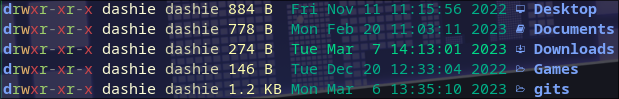
\includegraphics[scale=0.4]{2023_03_07_05_32_03.png}\newline
\textcolor{purple}{These rights are also stored as Macros in POSIX -> "sys/stat.h"}\newline
These can be chained with | -> S\_IRWXU | S\_IRGRP

\section{File API}
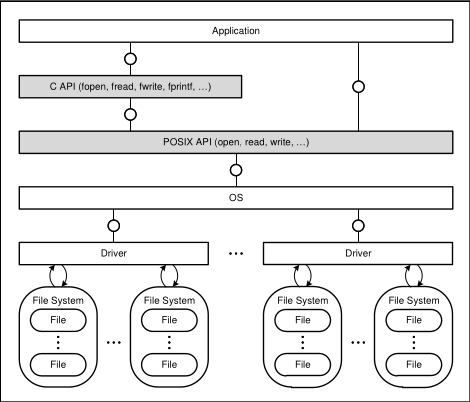
\includegraphics[scale=0.4]{2023_03_07_05_43_05.png}
\textcolor{purple}{The main difference with the POSIX API to the C API, is that the POSIX API gives us raw data, without any interpretation of the data, while the C API supports more specific things such as sockets, decoding etc.}

\subsection{POSIX File API}
General Info:
\begin{itemize}
\item \textcolor{purple}{All file functions are declared in <unistd.h> and <fcntl.h>}
\item \textcolor{purple}{error codes can be checked with "errno"}
\item \textcolor{purple}{raw data}
\item \textcolor{purple}{should only be used for binary data, not for anything that needs interpretation}
\end{itemize} 

\subsubsection{Usage of errno}
\begin{lstlisting}
if (chdir("docs") < 0) { // type is int
  if (errno == EACCESS) { // EACCESS defined in the function documentation
    printf ("Error: %s\n", strerror (errno));
    // or you can use perror
    perror ("Error"); // this makes use of the standard error stream
  }
}
\end{lstlisting}
Note, not all function set this flag, and should be used immediately, as other function will overwrite it.\newline
\textcolor{teal}{Codes for the error are directly defined in the function documentation.}\newline
\textcolor{purple}{Returns the address of a string, which describes the code in text.}\newline
perror is the same as strerror but with a special error stream.

\subsubsection{File-Descriptor}
\begin{itemize}
\item \textcolor{purple}{valid within a process}
\item \textcolor{purple}{indexed in a table of all open files in a process}
\item \textcolor{purple}{Process file table is indexed in the global table of all open files}
\item \textcolor{purple}{Receives data in order to identify physical file (correct hardware with correct driver)}
\item \textcolor{purple}{State defined: knows current offset (offset of byte that will be read next)}
\end{itemize} 
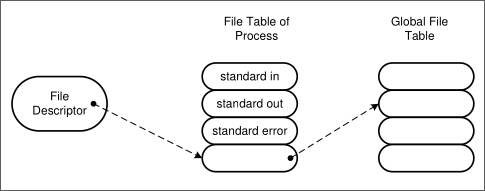
\includegraphics[scale=0.4]{2023_03_07_06_03_34.png}\newline
\textcolor{purple}{In each process open file index for a process there are 3 predefined file descriptors}\newline
\begin{lstlisting}
// STDIN_FILENO = 0  -> standard input
// STDOUT_FILENO = 1 -> standard output
// STDERR_FILENO = 2 -> standard error
\end{lstlisting}

\subsubsection{Opening files with POSIX API}
\begin{lstlisting}
int open (char *path, int flags, ...)
\end{lstlisting}
\begin{itemize}
\item \textcolor{black}{O\_RDONLY:} Read only
\item \textcolor{black}{O\_RDWR:} read and write
\item \textcolor{black}{O\_CREAT:} create file if not exists, needs another parameter for access rights
\item \textcolor{black}{O\_APPEND:} set offset to end of file before each write access
\item O\_TRUNC: set length of file to 0
\end{itemize} 

\subsubsection{Close files with POSIX API}
\begin{lstlisting}
int close(int fd)
\end{lstlisting}
deallocates file descriptor fd, which can now be used by other functions.\newline
returns 0 if ok, and -1 for error

\subsubsection{Usage of open and close}
\begin{lstlisting}
int fd = open("filename.file", O\_RDONLY);
if (fd < 0) {
  // le error handling
}
// do something with file
close(df);
\end{lstlisting}

\subsubsection{Read data with POSIX API}
\begin{lstlisting}
ssize_t read (int fd, void *buffer, size_t n)
// ssize_t is a signed size_t
\end{lstlisting}
\begin{itemize}
  \item tries to copy the next n(parameter) bytes to current offset from fd to the buffer 
\item returns count of read bytes or -1 when error
\item blocks thread until: n bytes are copied, error occurs, end of file has been reached
\item increments offset of fd by the amount of read bytes
\end{itemize} 

\subsubsection{Write data with POSIX API}
\begin{lstlisting}
ssize_t write (int fd, void *buffer, size_t n)
// ssize_t is a signed size_t
\end{lstlisting}
\begin{itemize}
  \item tries to copy the n bytes from the buffer to the offset on fd 
\item returns count of written bytes or -1 on error
\item blocks thread until n bytes are written, error occurs, or the end of file has been reached
\item increments offset of fd by the amount of bytes written
\end{itemize} 
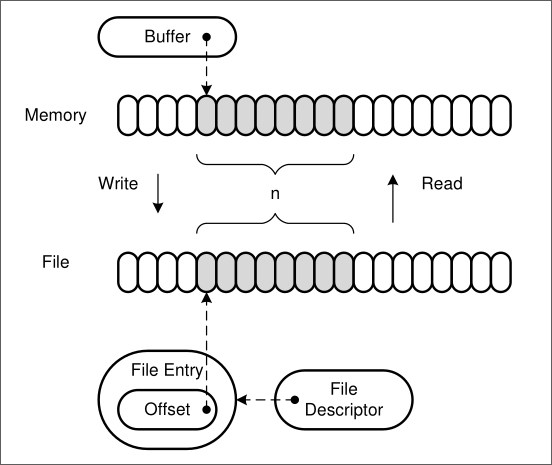
\includegraphics[scale=0.4]{2023_03_07_06_18_08.png}

\subsubsection{Jump in a file with POSIX API}
\begin{lstlisting}
off_t lseek (int fd, off_t offset, int origin)
\end{lstlisting}
\begin{itemize}
\item parameter offset that should be the new offset of fd
\item origin = SEEK\_SET for start of file
\item origin = SEEK\_CUR for current offset
\item origin = SEEK\_END for end of file
\item returns new offset or -1 on error
\end{itemize} 
Example usage:
\begin{lstlisting}
lseek (fd, 0, SEEK_CUR) return current offset
lseek (fd, 0, SEEK_END) return size of file
lseek (fd, n, SEEK_END) go beyond end of file, which will make write put 0s in this space if called. 
\end{lstlisting}
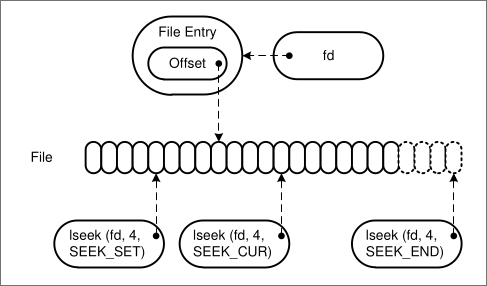
\includegraphics[scale=0.4]{2023_03_07_06_22_16.png}

\subsubsection{pread and pwrite in POSIX API}
\begin{lstlisting}
ssize_t pread (int fd, void *buffer, size_t n, off_t offset)
ssize_t pwrite (int fd, void *buffer, size_t n, off_t offset)
\end{lstlisting}
\textcolor{purple}{These are alternatives to write and read, that do not change the offset, however, this means that you will need to define where we are currently!}

\subsubsection{windoof proprietary paths}
\begin{itemize}
  \item \textbackslash instead of / because fuck you
  \item \textbackslash also needs to be escaped if you want to write it
\item root directory per disk instead of per system
\item C is the default disk, A and B were reserved for floppy disks
\item functions in windoof: \newline
  \begin{itemize}
  \item \textcolor{black}{open -> CreateFile}
  \item \textcolor{black}{read -> ReadFile}
  \item \textcolor{black}{write -> WriteFile}
  \item \textcolor{black}{lseek -> SetFilePointer}
  \item close -> CloseHandle
  \end{itemize} 
\end{itemize} 

\subsubsection{Example for reading and writing data in POSIX API}
\begin{lstlisting}
#define N 32
char buf[N];
char spath[PATH_MAX];
char dpath[PATH_MAX];

/* get paths from somewhere */

int src = open(spath, O_RDONLY);
int dst = open(dpath, O_WRONLY | O_CREAT, S_IRWXU);
ssize_t read_bytes = read(src, buf, N);
write(dst, buf, read_bytes);
close(src);
close(dst);
\end{lstlisting}

\subsection{C Stream API}
Idea: Operating systems do things differently, even something as simple as a newline is handled differently, so we need an API that can translate this to the correct symbol:\newline
\begin{lstlisting}
// Windows: \r \n = 13d 10d = 0Dh 0Ah
// Linux: \n = 10d = 0Ah
// Mac OS: \r = 13d = 0Dh (before Mac OSX, now just like penguinOS)
\end{lstlisting}
\begin{itemize}
\item \textcolor{purple}{OS independent}
\item \textcolor{purple}{stream-based: symbol-oriented}
\item \textcolor{purple}{can be buffered or unbuffered}\newline
  dependent on the implementation, transparent for applications
\item \textcolor{purple}{normally buffered for files}\newline
  independently transfers data-blocks between files and buffers
\item \textcolor{purple}{Has a file Position indicator}\newline
  - for buffered streams: defines position in buffer\newline
  - for unbuffered streams: is the offset in the file-descriptor
\end{itemize} 

\subsubsection{FILE datastructure}
\begin{itemize}
\item \textcolor{purple}{has information about a stream}
\item \textcolor{purple}{should not be used directly, instead only per pointers that are created via the C-API}
\item \textcolor{purple}{should not be copied, pointer can be used as ID by the API}
\item \textcolor{purple}{three predefined standard-streams}\newline
  \begin{itemize}
  \item \textcolor{black}{FILE *stdin}
  \item \textcolor{black}{FILE *stdout}
  \item \textcolor{black}{FILE *stderr}
  \end{itemize} 
\end{itemize} 

\subsubsection{open file with C-API}
\begin{lstlisting}
FILE * fopen (char const *path, char const *mode)
// flags
// "r": like O_RDONLY
// "w": like O_WRONLY | O_CREAT | O_TRUNC
// "a": like O_WRONLY | O_CREAT | O_APPEND
// "r+": like O_RDWR
// "w+": like O_RDWR | O_CREAT | O_TRUNC
// "a+": like O_RDWR | O_CREAT | O_APPEND
\end{lstlisting}
\begin{itemize}
\item \textcolor{black}{creates FILE-Object and stream for the file}
\item \textcolor{black}{returns pointer to created FILE-Object or 0 on error}
\end{itemize}

\subsubsection{close file with C-API}
\begin{lstlisting}
int fclose (FILE *file)
\end{lstlisting}
\begin{itemize}
\item \textcolor{black}{calls fflush}
\item \textcolor{black}{closes stream defined by file parameter}
\item \textcolor{black}{removes file from memory}
\item \textcolor{black}{returns 0 when ok, otherwise EOF}
\end{itemize} 

\subsubsection{flush of file with C-API}
\begin{lstlisting}
int fflush (FILE *file)
\end{lstlisting}
\begin{itemize}
\item \textcolor{black}{writes content to write from memory into file (if content exists)}
\item \textcolor{black}{will automatically be called when the buffer is full or file is closed}
\item \textcolor{black}{returns 0 when of, otherwise EOF}
\end{itemize} 

\subsubsection{Conversion from POSIX-API to C-API}
\begin{lstlisting}
FILE * fdopen (int fd, char const *mode)
// like fopen, but instead of path, we use a file descriptor

int fileno (FILE *stream)
// returns file-descriptor for the stream, or -1 on error
\end{lstlisting}

\subsubsection{read from file with C-API}
\begin{lstlisting}
int fgetc (FILE *stream)
\end{lstlisting}
\begin{itemize}
  \item \textcolor{black}{reads the next byte from stream \emph{as unsigned char} and returns it as int}
\item \textcolor{black}{increments the file-position indicator by 1}
\end{itemize} 
\begin{lstlisting}
char * fgets (char *buf, int n, FILE *stream)
\end{lstlisting}
\begin{itemize}
\item \textcolor{black}{reads to n-1 symbols from stream, or until newline or EOF}
\item \textcolor{black}{adds a 0 and creates a null terminated string}
\item \textcolor{black}{returns buffer(string) or 0 on error}
\item \textcolor{black}{increments the file-position indicator by the amount of read symbols}
\end{itemize} 

\subsubsection{"un"read from file with C-API}
\begin{lstlisting}
int ungetc (int c, FILE *stream)
\end{lstlisting}
\begin{itemize}
  \item \textcolor{black}{puts c(parameter -> file-descriptor) back to the stream into a special \emph{unget stack}}
\item \textcolor{black}{the next fget call will prefer the symbols in the unget stack}
\item \textcolor{black}{no change in the file itself}
\item \textcolor{black}{unget stack has a minimum size of 1 -> works at least once, can work multiple times depending on implementation}
\item returns c(parameter -> file-descriptor) or EOF on error
\end{itemize} 
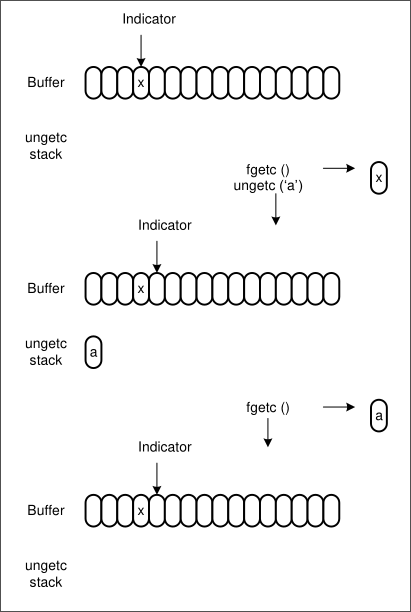
\includegraphics[scale=0.4]{2023_03_07_07_10_15.png}

\subsubsection{Write to file with C-API}
\begin{lstlisting}
int fputc(int c, FILE *stream)
\end{lstlisting}
\begin{itemize}
\item \textcolor{black}{converts file-descriptor c in unsgined char and writes it to stream}
\item \textcolor{black}{returns either c or EOF}
\item \textcolor{black}{increments the file-position indicator by 1}
\end{itemize} 
\begin{lstlisting}
int fputs (char *s, FILE *stream)
\end{lstlisting}
\begin{itemize}
\item \textcolor{black}{writes the symbols from the string s until the 0 termination symbol into the stream}
\item \textcolor{black}{the 0 termination will not be written}
\item \textcolor{black}{returns EOF on error}
\end{itemize} 

\subsubsection{End of file and Error in File C-API}
\begin{lstlisting}
int feof (FILE *stream)
// returns 0 when end of file has NOT been reached

int ferror (FILE *stream)
// retuns 0 when NO error occurred

// Example usage:
int return_value = fgetc (stream);
if (return_value == EOF) {
  if (feof (stream) != 0) {
    /* EOF reached */
  } else if (ferror (stream) != 0) {
    /* error occurred, check errno */
  }
}
\end{lstlisting}

\subsubsection{Manipulation of file-position indicator with C-API}
\begin{lstlisting}
long ftell (FILE *stream)
// returns the current file-indicator
// POSIX extension of ftello with return type off_t

int fseek (FILE *stream, long offset, int origin)
// set the file-position indicator like lseek
// POSIX extension of fseeko with off_t as type for the offset

int rewind (FILE *stream)
// reset the stream
// equivalent to fseek(stream, 0, SEEK_SET) and clear the error state
\end{lstlisting}


\subsection{Ext2}

\subsection{Ext4}

\section{Processmodels}
\subsection{Base}
Whenever we run a program, there are at least 2 actors: the program itself and the OS.\newline
The communication between OS and program runs on the C-API (or soon rust as well :) )\newline
Each program only knows itself and the OS.\newline
\textcolor{teal}{Systems like this are called \emph{monoprogramming}}

\subsubsection{Improvement with "async"}
This is what javascript does, it is only pseudo parallel in the sense that there is \emph{efficient process switching}, however we are still at 1 process at a time!\newline
There are multiple names for a process in this case -> task, job, or simply process. \newline
\textcolor{teal}{Here we still want to ensure that each program may think that is "the only running program",\newline
this means that the operating system \emph{must provide each service individually} -> memory, IO, etc. }

\subsection{Process}
\minipg{
  Each process has:
\begin{itemize}
\item \textcolor{purple}{Text section: image of the program in the memory (binary)}
\item \textcolor{purple}{data section: global variables of the program}
\item \textcolor{purple}{memory for heap}
\item \textcolor{purple}{memory for stack}
\end{itemize} 
}{
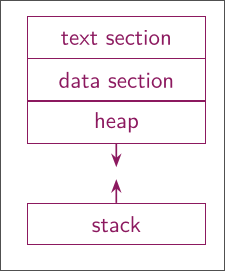
\includegraphics[scale=0.4]{2023_03_21_05_18_00.png}
}[0.25,0.25]

\subsubsection{Program vs Process}
\minipg{
Process
\begin{itemize}
\item \textcolor{purple}{active: actually executes instructions}
\item \textcolor{purple}{executes instructions in serial manner}
\item \textcolor{purple}{may perform actions for multiple programs -> according to POSIX}
\end{itemize} 
}{
Program
\begin{itemize}
\item \textcolor{purple}{passive: only says what to do}
\item \textcolor{purple}{can be run in parallel -> multiple processes execute different tasks for the program}
\end{itemize} 
}[0.25,0.25]

\subsubsection{Process Control Block (PCB)}
\textcolor{purple}{The operating system stores information about a process in this block.}
\begin{itemize}
\item \textcolor{purple}{ID for process -> PID}
\item \textcolor{purple}{Memory for the state of the processor}
\item \textcolor{purple}{scheduling information}
\item \textcolor{purple}{data for synchronization and communication between processes}
\item \textcolor{purple}{filesystem relevant information -> current open files}
\item \textcolor{purple}{Security-information}
\end{itemize} 
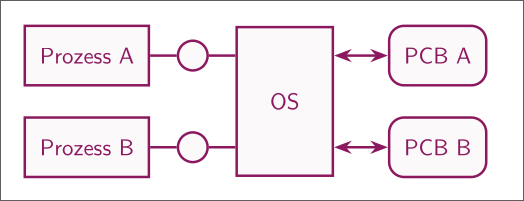
\includegraphics[scale=0.4]{2023_03_21_05_24_50.png}

\subsubsection{Interrupts, Processes and Context Switch}
\textcolor{teal}{For every interrupt the Operating system saves the current state of the process in the PCB.}\newline
The following will be saved:
\begin{itemize}
\item \textcolor{black}{Registers}
\item \textcolor{black}{Flags}
\item \textcolor{black}{Instruction Pointer}
\item \textcolor{black}{MMU-Configuration -> Page-Table-Pointer}
\end{itemize} 
\textcolor{teal}{After that, the interrupt handler will be called (which is run by the OS), which can switch context if needed -> e.g. switch to another process.\newline
As soon as the handler is done, the new context PCB is recovered.}

\subsubsection{Creation of a process}
\minipg{
POSIX:
\begin{enumerate}
\item \textcolor{purple}{create process}
\item \textcolor{purple}{load a program into this process and put it into ready mode}
\end{enumerate} 
}{
  Windoof:\newline
  both at once... (proprietary)
}[0.25,0.25]

\subsection{Process Hierarchy}
In POSIX, each process has exactly 1 parent, other than the root process.\newline
Each process can have unlimited amount of child processes!\newline
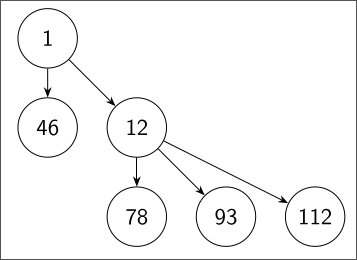
\includegraphics[scale=0.4]{2023_03_21_05_31_06.png}

\subsubsection{fork function}
The fork funcion crates an exact copy of the parent process.
\begin{lstlisting}
pid_t fork(void)
// not to mistake with :(){ :|:& };:
// kekw
\end{lstlisting}
\begin{itemize}
\item \textcolor{black}{the forked process has its own ID -> PID}
\item \textcolor{black}{the forked process has the parent ID saved as well}
\item the return of this function will be handled in \emph{both processes}\newline
  in parent: return will be either the ID or -1 for error\newline
  in child: returns 0
\end{itemize} 
Example of usage:
\begin{lstlisting}
int main() {
  pid_t new_pid = fork()
  // from here on both processes run this.

  if (new_pid > 0) {
    // this is the parent process
    // only the parent will run here
  } else if (new_pid == 0) {
    // this is the child process
    // only the child will run here
  } else {
    // error handling for parent process if forking failed
  }
}
\end{lstlisting}

\subsubsection{exit function}
\begin{lstlisting}
void exit(int code)
\end{lstlisting}
This is a return method to get out of a process.\newline
The code is simply the error handling code that you would like to pass to the parent process.

\subsubsection{wait function}
\begin{lstlisting}
pid_t wait(int* status)
\end{lstlisting}
\begin{itemize}
  \item \textcolor{black}{blocks process until \emph{one of his child processes ends}}
\item \textcolor{black}{the status will cover the return code of the child process}
\item \textcolor{black}{status usually handled with macros:}\newline
  WIFEXITED(*status) != 0 -> if child exited properly \newline
  WEXITSTATUS(*status): exit code of child
\item \textcolor{black}{will return -1 if error}\newline
  ECHILD: no child anymore to wait for (if false you still have children)\newline
  EINTR: was interrupted by signal
\end{itemize} 

\subsubsection{waitpid function}
\begin{lstlisting}
pid_t waitpid (pid_t pid, int *status, int options)
\end{lstlisting}
Like wait, but you can choose the child to wait for with pid.
\begin{itemize}
\item \textcolor{black}{pid > 0: waits for child with this pid}
\item \textcolor{black}{pid == -1: waits for any child -> like wait}
\item \textcolor{black}{pid == 0 and pid < -1 enables waiting for processes of a specific process group}
\end{itemize} 

\subsubsection{Examples}
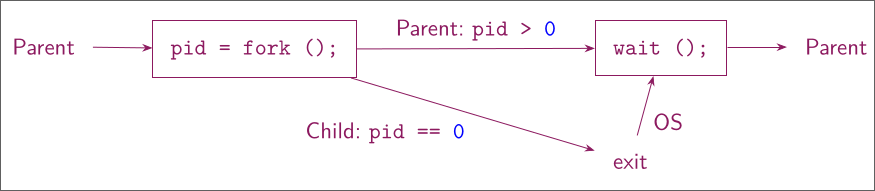
\includegraphics[scale=0.4]{2023_03_21_05_59_40.png}\newline
Worker example:
\begin{lstlisting}
#include <stdio.h>
#include <stdlib.h>
#include <sys/types.h>
#include <unistd.h>
#include <errno.h>
#include <sys/wait.h>

void spawn_worker(int a) {
  if (fork() == 0) {
    // we are in child
    printf("%d",a);
    // print number of process
    exit(0); // return code ok
  }
}

int main() {
  int pid = 0;
  for (int i = 0; i < 10; i++) {
    spawn_worker(i);
    // create 10 child processes
  }

  // do something in parent

  do {
    pid = wait(0);
    // status code is not saved!
  }

  while (pid > 0 || errno != ECHILD);
  // run until no more children!
}
\end{lstlisting}

\subsubsection{exec functions}
\textcolor{teal}{There are 6 versions of exec -> execl, execle, execlp, execv, execve, execvp}\newline
Each exec function \emph{replaces the program in the current process with another}.\newline
Parameters:
\begin{itemize}
\item \textcolor{black}{execl*: binary and args as list -> execl(path0, arg0, arg1, ...)}
\item \textcolor{black}{execv*: binary and args as vector -> execv(path, argv)}
\item \textcolor{black}{exec*e: allow array for environment variables as parameter, in the other variants the env-vars stay the same}
\item \textcolor{black}{exec*p: search for filename via environment variable PATH, the others use absolute or relative paths}
\end{itemize} 
\textcolor{teal}{the * means any character -> functions are a family}\newline
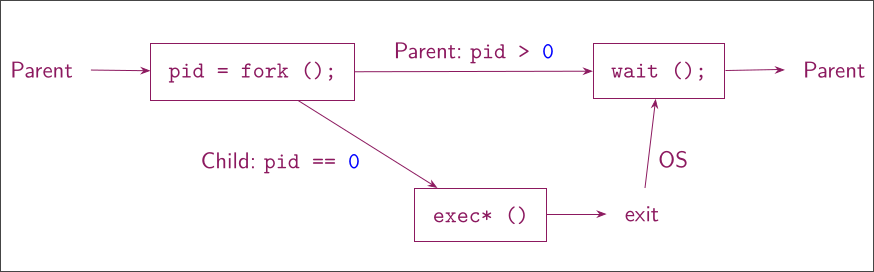
\includegraphics[scale=0.4]{2023_03_21_06_15_17.png}

\subsubsection{Zombie Processe}
\textcolor{purple}{This refers to child processes that have ended, but aren't removed yet.\newline
This means the PCB etc are all still there, but it doesn't do anything.\newline
This stays like this until the parent calls wait() for this child!}\newline
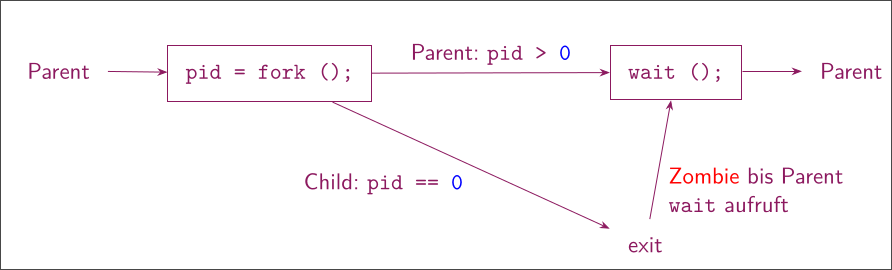
\includegraphics[scale=0.4]{2023_03_21_06_18_24.png}

\subsubsection{Orphan Process}
\textcolor{purple}{This is even worse than regular zombie processes. This means that the parent process is now dead, therefore no process can wait for this.\newline
The only solution here is an operating system process with the pid1, this process will inherit these child processes and will then continuously end all of them.}\newline
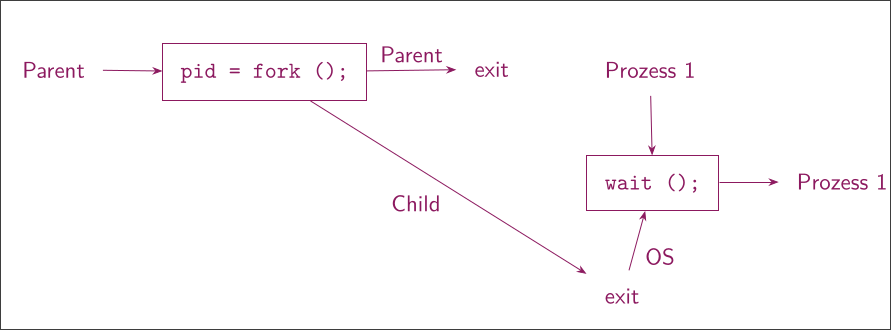
\includegraphics[scale=0.4]{2023_03_21_06_20_43.png}\newline
Note, it might be that the parent process is stuck/has an error, in this case the child processes will be passed to 1 for ending them, while the parent is killed.

\subsubsection{function sleep}
\begin{lstlisting}
unsigned int sleep(unsigned int seconds)
\end{lstlisting}
\begin{itemize}
\item \textcolor{black}{waits "closesly" for the amount of seconds provided}
\item \textcolor{black}{can be interrupted by the OS (example: signals)}
\item \textcolor{black}{returns the amount of seconds that would remain to sleep}\newline
  example if interrupted after 5 seconds, returns entered time - 5 seconds
\end{itemize} 

\subsubsection{function atexit}
\textcolor{teal}{Here you can pass functions that will be executed before the process exits.\newline
This is usefull for resources that the OS doesn't know/care about.}
\begin{lstlisting}
int atexit(void (*function)(void))
\end{lstlisting}
\begin{itemize}
\item \textcolor{black}{atexit can be called multiple times to register multiple functions}
\item \textcolor{black}{same function can be registered multiple times}
\item \textcolor{black}{functions will be called in reverse order to registered order!}
\end{itemize} 

\subsubsection{function to read pid}
These functions simply return the pid of the current process or the parent.
\begin{lstlisting}
#include <stdio.h>
#include <unistd.h>
int main() {
  pid_t my_pid = getpid();
  pid_t my_parent_pid = getppid();
  // do something with pid
}
\end{lstlisting}

\section{C Toolchain}
The toolchain handles the \emph{precompilation, compilation, assembling and linking} of executables.

\subsection{Precprocessor}
The preprocessor translates Macros and header files into actual code.\newline
The output will then be passed to the translation unit and the compiler.

\subsection{Linker}
After the individual assembly files have been assembled, the linker takes all object files and creates one executable from them.

\subsection{Loader}
\textcolor{teal}{The loader takes executables and dynamic libraries and loads them into ram.\newline
Note that static libraries are basically inside the executable.}\newline

\includegraphics[scale=0.4]{2023_03_28_05_13_22.png}

\subsubsection{Penguin Loader}
The loader under linux has the following steps: 
\begin{enumerate}
\item \textcolor{black}{exec* have syscalls on sys\_execve}
\item \textcolor{black}{searches for file, checks for permission and opens specified file}
\item \textcolor{black}{counts and copies arguments and environment variables}
\item \textcolor{black}{provides request for each registered "binary handler"}
\item Binary handler try to load data and interpret data one by one
\item program is now executed
\end{enumerate} 
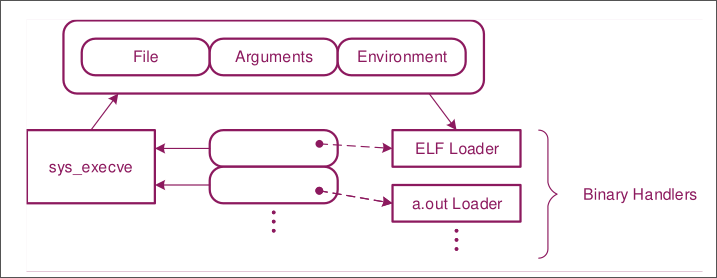
\includegraphics[scale=0.4]{2023_03_28_05_16_35.png}

\subsection{Executable Linking Format ELF}
\begin{itemize}
\item \textcolor{black}{Binary format, which specifies a program as binary}\newline
  windoof and penguin have some more than just this
\item \textcolor{black}{two possible formats}\newline
  Linking view\newline
  Execution view
\item \textcolor{black}{Used for linker and loader}\newline
  Object-File: Linking-view -> something.o
  Programs: Execution-view -> no ending?
  Shared-Objects: dynamic libraries (Linking and Execution View!) -> wlroots.so
\item \textcolor{black}{item 4}
\end{itemize} 

\subsubsection{ELF Structure}
\minipg{
\begin{itemize}
\item \textcolor{black}{Header}
\item \textcolor{black}{Program Header Table: (only necessary in execution view)}
\item \textcolor{black}{Segments: (only necessary in execution view)}
\item \textcolor{black}{Section: Header Table (only necessary in linking view)}
\item Sections: (only necessary in linking view)
\end{itemize} 
}{
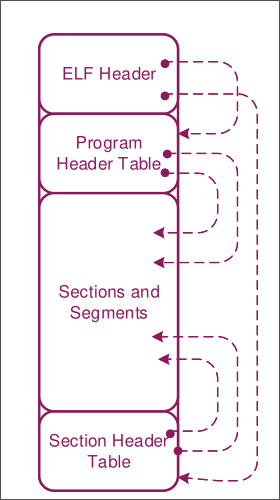
\includegraphics[scale=0.4]{2023_03_28_05_20_06.png}
}[0.25,0.25]

\subsubsection{Segments and Sections}
\minipg{
\begin{itemize}
\item \textcolor{purple}{Segments and sections occupy the same memory space}\newline
  Compiler specifies space for sections\newline
  Linker specifies space for segements
\item \textcolor{purple}{Linker combines segments with the same names and defines segments}
\item \textcolor{purple}{Compiler defines sections}
\end{itemize} 
}{
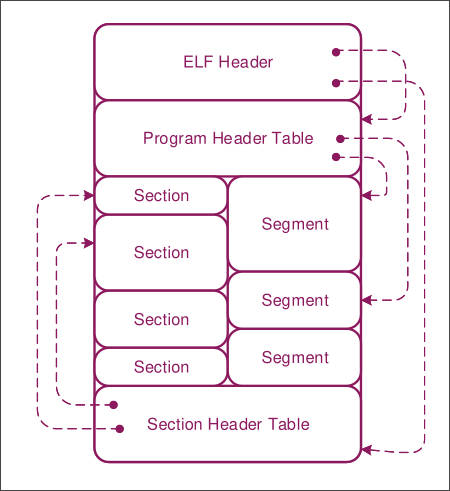
\includegraphics[scale=0.4]{2023_03_28_05_20_40.png}
}[0.25,0.25]

\subsubsection{Header of an ELF file}
\begin{itemize}
\item \textcolor{black}{52 byte: describes the structure of the file}
\item \textcolor{black}{Type: Reallocatable, executable, shared object?}
\item \textcolor{black}{32 or 64 bit}
\item \textcolor{black}{Encoding: little or big endian}
\item Machine: i386, arm, intel 64 etc
\item Entrypoint: Address at which the program should start -> main()
\item relative address, count and size of the entries for the program header table
\item relative address, count and size of the entries for the section header table
\end{itemize} 

\subsubsection{Program Header Table and Segments}
\begin{itemize}
\item \textcolor{black}{Program Header Table (or Segment Header Table): Table with n entries}
\item \textcolor{black}{Each entry is 32 bit and describes a segment}\newline
  \begin{itemize}
  \item \textcolor{black}{Segment-Type and Flags}
  \item \textcolor{black}{Offset and size of file}
  \item \textcolor{black}{Virtual address and size in memory -> possible addition: physical address}
  \end{itemize} 
\item \textcolor{black}{Segments are used at runtime by the loader}\newline
  Loader loads specified segments to memory\newline
  Loader may use more segments for other purposes: dynamic linking
\end{itemize} 
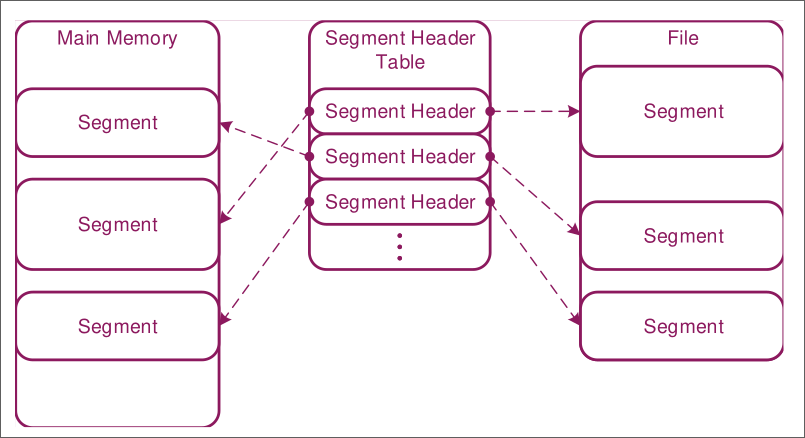
\includegraphics[scale=0.4]{2023_03_28_05_31_42.png}

\subsubsection{Sections}
\begin{itemize}
\item \textcolor{black}{Section Header Table: Table with m entries (usually :m != n | not equal sections to segments)}
\item \textcolor{black}{Each entry (40bytes) describes a section}\newline
  \begin{itemize}
  \item \textcolor{black}{Reference to string table }
  \item \textcolor{black}{Type and Flags}
  \item \textcolor{black}{Offset and Size of file}
  \item \textcolor{black}{Specific information based on section type}
  \end{itemize} 
\item \textcolor{black}{Sections will be used by linker}\newline
  \begin{itemize}
  \item \textcolor{black}{collects and concatenates(same name) sections of all object files}
  \item \textcolor{black}{generates executable}
  \end{itemize} 
\end{itemize} 
\textcolor{teal}{Section Types}
\begin{itemize}
\item \textcolor{purple}{SHT\_PROGBITS}Data defined by program, linker does not interpret this
\item \textcolor{purple}{SHT\_SYMTAB}Symbol Table
\item \textcolor{purple}{SHT\_STRTAB}String Table
\item \textcolor{purple}{SHT\_REL/RELA}Relocation Information
\item \textcolor{purple}{SHT\_HASH}Hashtable for symbols
\item \textcolor{purple}{SHT\_DYNAMIC}Information for dynamic Linking
\item \textcolor{purple}{SHT\_NOBITS}Setion without data in file
\end{itemize} 
\textcolor{teal}{Section Attributes}
\begin{itemize}
\item \textcolor{purple}{SHF\_WRITE} data of this section should be writable during execution
\item \textcolor{purple}{SHF\_ALLOC} data of this section should be in memory during execution
\item \textcolor{purple}{SHF\_EXECINSTR} data of this section display machine code
\end{itemize} 
\textcolor{teal}{Special Sections}
\begin{itemize}
  \item \textcolor{purple}{.bss:} uninitialized data
  \item \textcolor{purple}{.data:} initialized data
  \item \textcolor{purple}{.data1:} initialized data
  \item \textcolor{purple}{.debug:} debug information
\item \textcolor{purple}{rodata:} read only data
\item \textcolor{purple}{.rodata1: } read only data
\item \textcolor{purple}{.text: } executable instructions 
\item \textcolor{purple}{.symtab: } Symbol-Table 
\item \textcolor{purple}{.strtab: } String-Table 
\end{itemize} 

\subsubsection{String Table}
\begin{itemize}
\item \textcolor{black}{Section of a file that has null terminated strings in a row}
\item Strign reference -> offset of string (starts at 0 and increases per char) 
\item \textcolor{black}{typically has names of symbols}
\item \textcolor{black}{typically does NOT include string literals like "henlo birb!", this is usually in .rodata}
\item \textcolor{black}{item 4}
\end{itemize} 
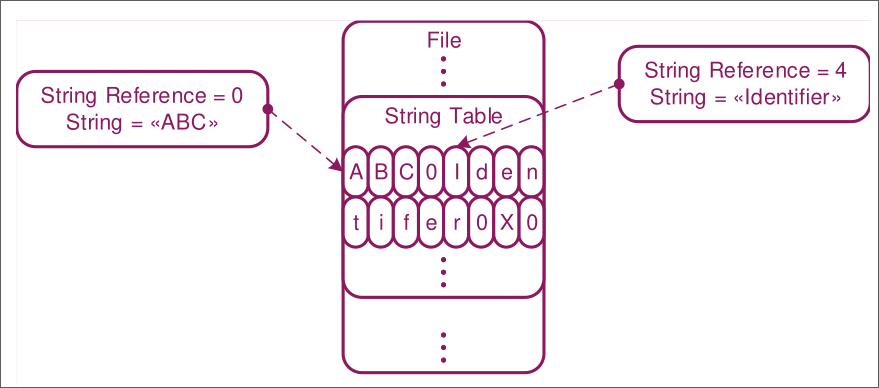
\includegraphics[scale=0.4]{2023_03_28_05_47_52.png}

\subsubsection{Symbols}
\begin{itemize}
\item \textcolor{black}{Symbol Table: each entry has 1 symbol}
\item \textcolor{black}{Symbol: 16 bytes}\newline
  \begin{itemize}
  \item \textcolor{black}{Name: 4 bytes, reference in string table}
  \item \textcolor{black}{Value: 4 bytes, depends on symbol type, could be an address for example}
  \item \textcolor{black}{Size: 4 bytes, size of symbol (for example length of function)}
  \item \textcolor{black}{Info: 4 bytes types, binding attributes (local, global, weak), reference to section header}
  \end{itemize} 
\end{itemize} 

\subsection{Static Libraries}
\begin{itemize}
\item \textcolor{black}{Static libraries are archives of object files}
\item \textcolor{black}{will be produced with the "ar" tool}
\item \textcolor{black}{named lib<something>.a -> note the ending}
\item \textcolor{black}{will only be referenced if included in compilation -> clang -lmylib}
\item static libraries are included in the binary and will receive a static address
\end{itemize} 
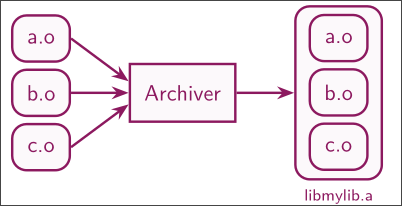
\includegraphics[scale=0.4]{2023_03_28_06_00_43.png}
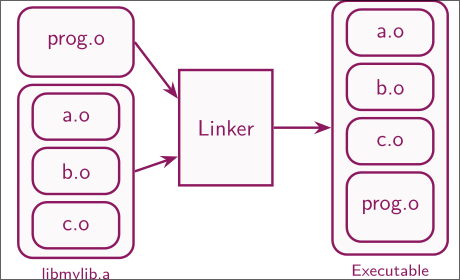
\includegraphics[scale=0.4]{2023_03_28_06_00_54.png}\newline
More information:
\begin{itemize}
\item \textcolor{black}{In the early days, there were only static libraries}
\item \textcolor{green}{Will never cause a program to suddenly stop working due to updates -> it is included in binary!}
\item \textcolor{green}{easy to implement and use}
\item \textcolor{red}{Must be recompiled with program if changes are made}
\item \textcolor{red}{increases binary size}
\item \textcolor{red}{functionality can't be increased with updates to library for binaries -> again must be recompiled}
  \item \textcolor{red}{plugins impossible or only very hard}
\end{itemize} 

\subsection{Dynamic Libraries}
\begin{itemize}
\item \textcolor{black}{loaded at runtime}
\item \textcolor{red}{harder to implement}
\item \textcolor{black}{executable receives only a reference to library}
\item \textcolor{green}{library can be updated independent of binary}
\item \textcolor{red}{if binary might stop working on library updates} 
\item \textcolor{green}{Plugins are relatively easy to create}\newline
  Create API
\end{itemize} 
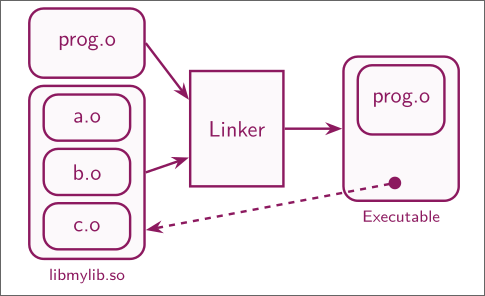
\includegraphics[scale=0.4]{2023_03_28_06_07_41.png}
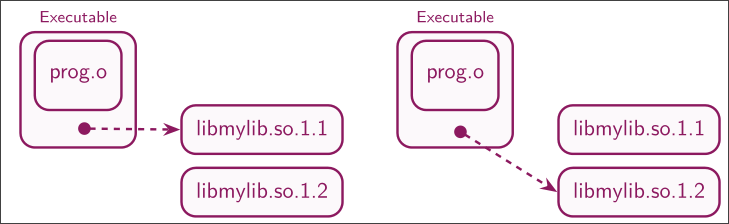
\includegraphics[scale=0.4]{2023_03_28_06_07_57.png}

\subsubsection{Delayed Loading}
\textcolor{teal}{This is essentially lazy loading for libraries, only the libraries that will be used right then and there are loaded in order to save memory.}
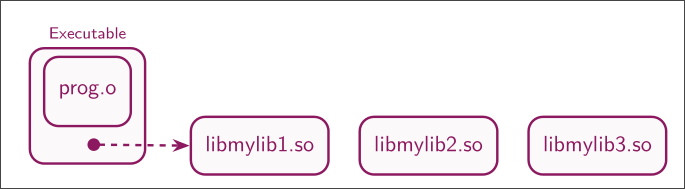
\includegraphics[scale=0.4]{2023_03_28_06_10_44.png}

\subsection{POSIX API: dynamic libraries}
\subsubsection{dlopen}
\textcolor{teal}{opens a dynamic library and returns a handle to it}
\begin{lstlisting}
void* dlopen(char* filename, int mode)
\end{lstlisting}
Mode specifies how to handle the file:
\begin{itemize}
\item \textcolor{black}{RTLD\_NOW: all symbols will be bound to the library on load}
\item \textcolor{black}{RTLD\_LAZY: symbols will be bound if needed}
\item \textcolor{black}{RTLD\_GLOBAL: } symbols can be bound used during binding of other object-files
\item \textcolor{black}{RTLD\_LOCAL: symbols can't be used for other object-files}
\end{itemize} 

\subsubsection{dlsym}
\textcolor{teal}{Returns the address of a symbol from the specified library (handle for library)}
\begin{lstlisting}
void* dlsym(void* handle, char* name)
\end{lstlisting}
\textcolor{teal}{There is no type information, you only receive an address.\newline
This means you can't know if it is a function, variable or whatever.}\newline
Example:
\begin{lstlisting}
typedef int (*func_t)(int);                // our function returns int and takes int
handle = dlopen ("libmylib.so", RTLD_NOW); // open dynamic library
func_t f = dlsym (handle, "my_function");  // take function from library and store in f
int *i = dlsym (handle, "my_int");         // take variable from library and store in i
(*f)(*i);                                  // call function
// Note we have no information about either f or i, we just assume they are function and variable respectively!
// You have to read API and documentation yourself to make sure that is the case!
\end{lstlisting}

\subsubsection{dlclose}
\textcolor{teal}{Closes the dynamic library via the specified library (handle to library)}
\begin{lstlisting}
  int dlclose(void* handle)
\end{lstlisting}
Returns 0 on success

\subsubsection{dlerror}
\textcolor{teal}{Returns a null terminated string as error if an error occurred.}
\begin{lstlisting}
  char* dlerror()
\end{lstlisting}

\subsubsection{Automatic Loading of ELF files}
As long as there is a reference to the library in the executable ELF file, libraries will automatically be loaded by need.

\subsection{Naming of Shared Objects}
\begin{itemize}
\item \textcolor{purple}{Linker-Name:} libmylib.so 
\item \textcolor{purple}{SO-Name:} libmylib.so.2
\item \textcolor{purple}{Real-Name (filename): } libmylib.so.2.1
\end{itemize} 
\textcolor{teal}{The tool "ldconfig" properly creates these files for you.}\newline
Usually only the realname exists, with the rest being \emph{soft-links}\newline
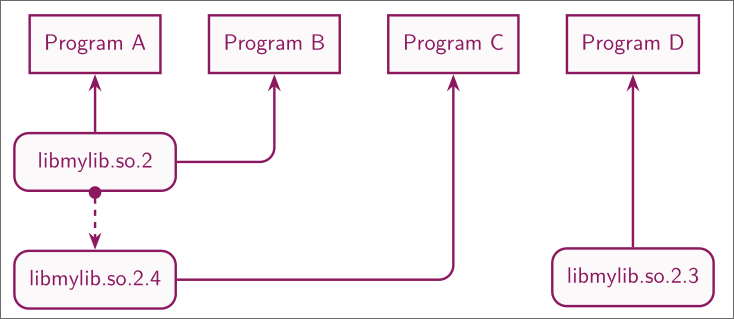
\includegraphics[scale=0.4]{2023_03_28_06_30_29.png}\newline
\textcolor{red}{As one can see, you should always use the SO name (or linker (not recommended)) at the least, if you link against the real name, then your application will break on each update...}

\subsubsection{Updates}
\begin{itemize}
\item \textcolor{black}{Real name never changes}
\item \textcolor{black}{SO-name: update on feature increases -> new API}
\item \textcolor{black}{Real-Name: update on bugfixes}
\end{itemize} 

\subsection{Shared Objects with Linker and Loader}
Linker uses the base name, the executable the SO name and the process will finally use the real name.\newline
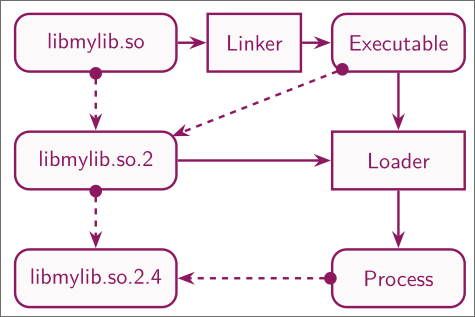
\includegraphics[scale=0.4]{2023_03_28_06_33_28.png}

\subsection{Creating Static Libraries:}
\begin{lstlisting}
// compile 
clang -c f1.c -o f1.o
clang -c f2.c -o f2.o

// create archive
ar r libmylib.a f1.o f2.o
\end{lstlisting}

\subsection{Creating Dynamic Libraries:}
\begin{lstlisting}
// compile
clang -fPIC -c f1.c -o f1.o
clang -fPIC -c f2.c -o f2.o

// create image -> .so file
clang -shared -Wl,-soname,libmylib.so.2 -o libmylib.so.2.1 f1.o f2.o -lc
\end{lstlisting}
\textcolor{red}{Important, the linker will prefer dynamic libraries, you need to override the default to use static versions if both exist}

\subsection{Using libraries}
\begin{lstlisting}
// static libraries
clang main.c -o main -L. -lmylib

// dynamic libraries
clang main.c -o main -lmylib

// dynamic library that will be called with dlopen
clang main.c -o main -ldl
\end{lstlisting}

\subsubsection{ld-linux.so effective loader}
\begin{itemize}
\item Can be used as an executable with --list flag
\item will be called by the OS indirectly
\item finds and loads all other shared objects one by one 
\item continues recursively to load all dependencies of loaded shared objects
\end{itemize} 
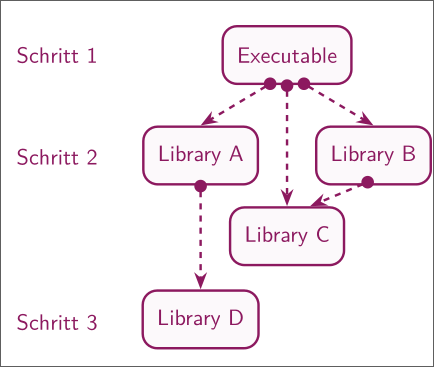
\includegraphics[scale=0.4]{2023_03_28_06_39_48.png}

\subsection{Shared Object Facts}
\begin{itemize}
\item \textcolor{black}{Referenced Shared Objects are stored inside the executables}\newline
  \begin{itemize}
  \item \textcolor{black}{readelf -d shows the content of dynamic section}
  \item \textcolor{black}{type of the entries is NEEDED}
  \end{itemize} 
\item \textcolor{black}{ldd shows all shared objects, even indrectly used ones}\newline
  \begin{itemize}
  \item \textcolor{black}{executes executables and instructs loader to show trace}
  \item \textcolor{black}{should only be used on trusted executables!!}
  \end{itemize} 
\item \textcolor{black}{Pretty much all Executables (C) need at least two shared objects}\newline
  \begin{itemize}
  \item \textcolor{black}{libc.so -> standard C library}
  \item \textcolor{black}{ld-linux.so -> ELF Shared Object Loader}
  \end{itemize} 
\end{itemize} 

\subsection{Dynamic Library Implementation}
Dynamic libraries must be able to be moved, this ofc since they are loaded into memory.\newline
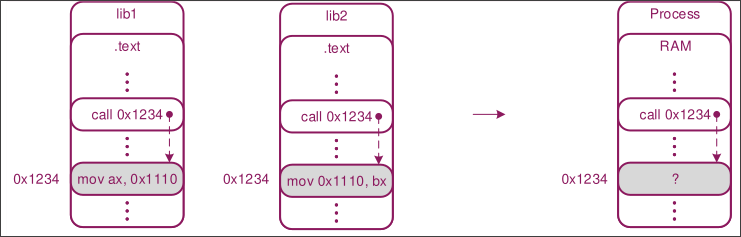
\includegraphics[scale=0.4]{2023_03_28_06_41_17.png}\newline
This however means that only one process at the time can load the library unless you load it twice, which is not something you want.\newline
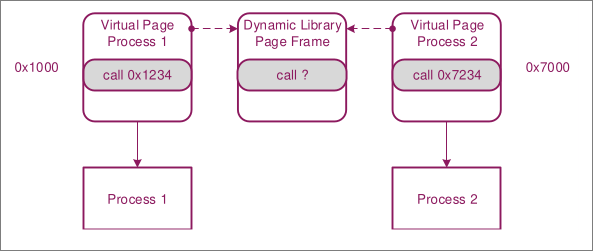
\includegraphics[scale=0.4]{2023_04_04_05_15_09.png}\newline
The solution to this is saving the address of the library which can be seen with 2 implementations below:

\subsubsection{Position-Dependent Code}
This means we jump to absolute addresses, in this case to absolute addresses of our dynamic library.\newline
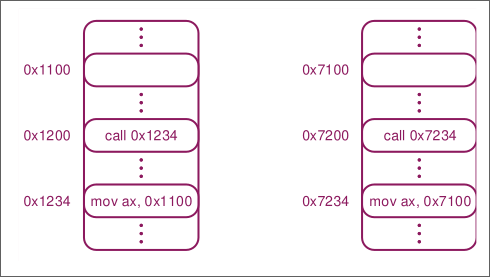
\includegraphics[scale=0.4]{2023_04_04_05_06_51.png}

\subsubsection{Position-Independent Code}
This means we jump relatively to our current instruction pointer inside of our program.\newline
\textcolor{teal}{Note that the CPU has to support this, 32bit for example does not.}\newline
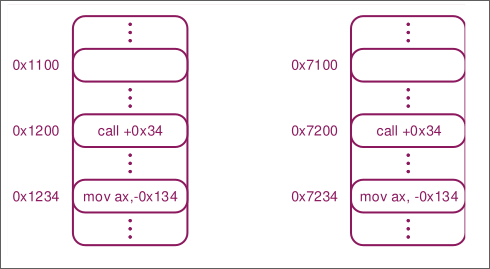
\includegraphics[scale=0.4]{2023_04_04_05_07_03.png}\newline

\subsubsection{Global Offset Table}
\minipg{
\textcolor{teal}{In each program/library we have a global offset table, which shows the relative distances to libraries etc that you need/want.\newline
This way you can use the same dynamic library that is loaded into memory, even though another process is also using it.}
}{
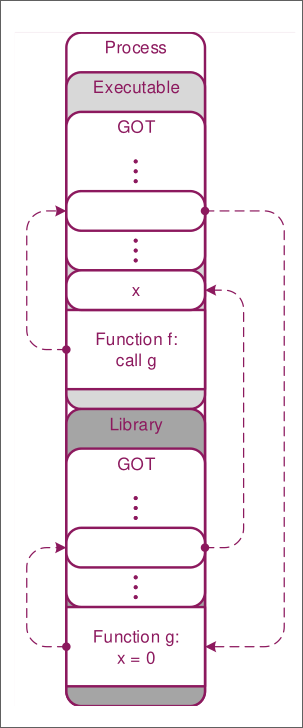
\includegraphics[scale=0.4]{2023_04_04_05_09_20.png}
}[0.5,0.25]

\subsection{PLT Process Linkage Table}
\textcolor{teal}{Implements lazy binding!}\newline
\begin{itemize}
\item \textcolor{black}{one function per entry}
\item \textcolor{black}{PLT entry has call instruction in GOT entry}
\item \textcolor{black}{GOT points to proxy function}
\item \textcolor{black}{Proxy function finds link to proper function and overwrites own entry}
\item \textcolor{green}{Benefit: eliminates check for "is it loaded" after initial load (is expensive!!)}
\end{itemize} 

\section{MultiThreading}

\subsection{Threads}
\begin{itemize}
\item \textcolor{purple}{Threads are parallel activities inside of a process}
\item \textcolor{purple}{Threads have equal access to all resources in the process}\newline
  \begin{itemize}
  \item code(text secion) 
  \item global variables (data section)
  \item heap
  \item open files
  \item MMU-data
  \end{itemize} 
\end{itemize} 

\subsection{Process-Model vs Thread-Model}
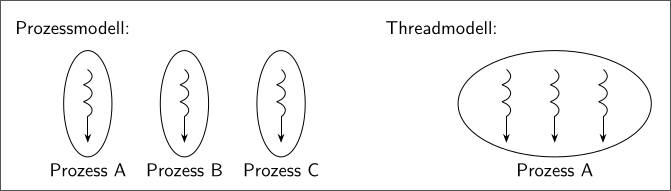
\includegraphics[scale=0.4]{2023_04_04_05_33_13.png}

\subsection{Thread as stack and context}
\minipg{
\begin{itemize}
\item \textcolor{black}{Each thread needs its own context and its own stack, since it will have its own function call stack}
\item \textcolor{black}{Information about call stack will usually be placed in a Thread-Control-Block}
\item \textcolor{black}{In Linux, each process has a copy of the Process-Control-Block of its own process instead!!}
\end{itemize} 
}{
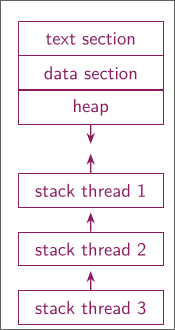
\includegraphics[scale=0.4]{2023_04_04_05_35_26.png}
}[0.25,0.25]
Example of two threads that call the same function:\newline
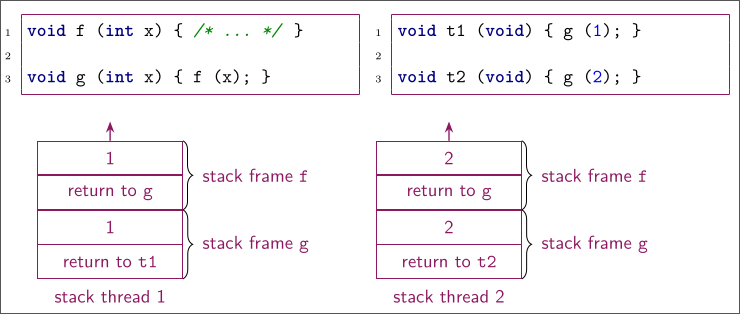
\includegraphics[scale=0.4]{2023_04_04_05_35_51.png}

\subsection{Parallization of algorithms}
\textcolor{teal}{Algorithms are by default serial, however, there are some parts that you could run in parallel.}\newline 
Example:
\begin{lstlisting}
// this can be split
for (int i = 0; i < n; ++i) {
  sum += a [i];
}

// into this
for (int i = 0; i < n / 2; ++i) {
  sum0 += a [i];
}
for (int i = n / 2; i < n; ++i) {
  sum1 += a [i];
}
sum = sum0 + sum1;
\end{lstlisting}

\subsubsection{Time difference}
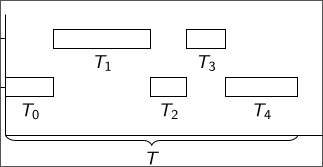
\includegraphics[scale=0.4]{2023_04_04_05_38_49.png}
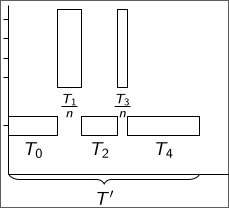
\includegraphics[scale=0.4]{2023_04_04_05_39_12.png}\newline
This shows the non parallizable parts on the bottom and the others on top.\newline
As it can be seen the top parts are shrinking by large margins since they can be done in parallel!\newline
\subsubsection{Speedup Factor}
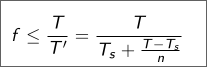
\includegraphics[scale=0.4]{2023_04_04_05_40_22.png}
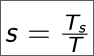
\includegraphics[scale=0.4]{2023_04_04_05_43_49.png}
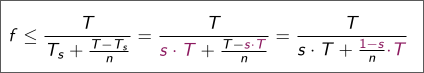
\includegraphics[scale=0.4]{2023_04_04_05_43_39.png}
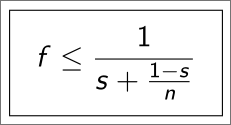
\includegraphics[scale=0.4]{2023_04_04_05_44_00.png}\newline
Legend:
\begin{itemize}
  \item \(f\): speedup factor 
\item \(T\): Total time
\item \(T'\): Time saved
\item \(T_s\): total time that must be done in serial fashion!
\item \(n\): Count of processors
\item \(s\): relation of serial time to total time\newline
  \textcolor{red}{Note this is often just a guess, not a calculation.\newline
  This is because we often can't say how long something would really take!}
\end{itemize} 

\subsection{Amdahls Rule}
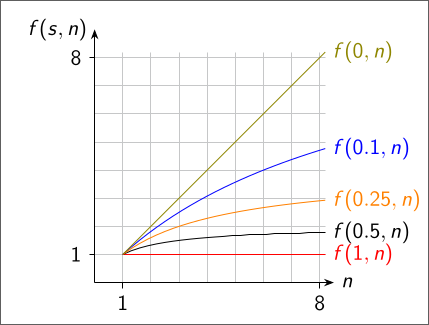
\includegraphics[scale=0.4]{2023_04_04_05_45_22.png}\newline
\textcolor{red}{f(s,n)!!}
\begin{itemize}
\item \textcolor{black}{best case: s==0 -> everything is parallelizeable}
\item \textcolor{black}{worst case: s==1 -> nothing is parallelizeable -> user input}
\end{itemize} 
If you keep increasing the processor count, then you will eventually go towards the limit of 1:\newline
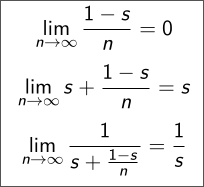
\includegraphics[scale=0.4]{2023_04_04_05_56_40.png}


\section{POSIX Threading API}
\subsection{Creating a thread}
\begin{lstlisting}
int pthread_create (
  pthread_t *thread_id,
  pthread_attr_t const *attributes,
  void * (*start_function) (void *),
  void *argument
)
\end{lstlisting}
\begin{itemize}
\item \textcolor{black}{Creates a thread and returns 0 on success, otherwise errorcode}
\item \textcolor{black}{The ID of the new thread will be stored in thread\_id}
\item \textcolor{black}{attributes is an opaque object, with which you can specify things like the stack-size}
\item start\_function is the first instruction the new thread will execute
\item the thread will place the parameter argument inside of that function
\item the programmer must ensure the start\_function and the argument are compatible
\item You must specify who is responsible for garbage collection of the data structure
\item \textcolor{red}{Don't delete the stack of the thread during its execution!}
\end{itemize} 

\subsubsection{Example for pthread}
\begin{lstlisting}
struct T {
  int value;
};

void *my_start(void * arg) {
  struct T* p = arg;
  printf ("%d\n", p->value);
  free (arg);
  return 0;
}

void start_my_thread (void) {
  struct T* t = malloc (sizeof(struct T));
  t->value = 109;
  pthread_t tid;
  pthread_create (
    &tid,
    0, // default attributes
    &my_start,
    t
  );
}
\end{lstlisting}
\textcolor{teal}{The default attributes are handled by the operating system!\newline
They are used when you pass 0 -> nullptr to this function}

\subsubsection{Attributes for pthread}
Attributes are handled the following way:
\begin{lstlisting}
pthread_attr_t attr;                       // variable for attribute
pthread_attr_init(&attr);                  // initialize attribute
pthread_attr_setstacksize(&attr, 1 << 16); // set the stacksize of attribute
pthread_create(..., &attr, ...);           // create attribute
pthread_attr_destroy(&attr);  );           // delete attribute
\end{lstlisting}
\textcolor{teal}{The number 0 means that we pass default attributes}

\subsection{pthread\_exit}
\begin{lstlisting}
void pthread_exit(void *return_value)
\end{lstlisting}
\begin{itemize}
\item \textcolor{black}{ends the thread and returns the return\_value}
\item \textcolor{black}{this is the equivalent to the return of the start\_function with a return value}
\end{itemize} 

\subsubsection{Lifetime of a thread}
A thread lives until:
\begin{itemize}
  \item \textcolor{black}{the thread executes a return statement}
\item \textcolor{black}{the thread calls pthread\_exit}
\item \textcolor{black}{another thread calls thread\_cancel}
\item \textcolor{black}{the thread is killed otherwise}
\end{itemize} 

\subsection{pthread\_cancel}
\begin{lstlisting}
int pthread_cancel(pthread_t thread_id)
\end{lstlisting}
\begin{itemize}
\item \textcolor{black}{Sends a demand to the OS to kill a thread with the thread\_id}
\item \textcolor{black}{The function doesn't wait for the thread to be killed}
\item \textcolor{black}{The return code is 0 when the thread exists, otherwise ESRCH errorcode}
\end{itemize} 

\subsection{pthread\_detach}
\begin{lstlisting}
int pthread_detach(pthread_t thread_id)
\end{lstlisting}
\begin{itemize}
\item \textcolor{black}{Removes the memory which a thread has allocated, as soon as the thread is terminated}
\item \textcolor{black}{Doesn't end the thread, in case the thread has not ended}
\item the return value is 0 if the thread exists, otherwise ESRCH
\end{itemize} 

\subsection{pthread\_join}
\begin{lstlisting}
int pthread_join(pthread_t thread_id, void **return_value)
\end{lstlisting}
\begin{itemize}
\item \textcolor{black}{waits until the thread\_id is dead}
\item \textcolor{black}{Takes the return value of the thread and stores it in the return\_value parameter}
\item \textcolor{black}{return\_value can be NULL -> 0, in this case it will not store the return value}
\item \textcolor{black}{calls pthread\_detach}
\item the return value is 0 if the thread exists, otherwise ESRCH
\end{itemize} 

\subsection{pthread\_self}
\begin{lstlisting}
pthread_t pthread_self(void)
\end{lstlisting}
Returns the ID of the current running thread

\section{Thread-Local Storage (TLS)}
The problem here is that there are certain things that are stored globally, take errno for example.\newline
If this would be thread overreaching, then another thread might overwrite errno, therefore interfering with another thread that is running somewhere else.\newline
This leads to race conditions where multiple threads want to access -> read/write this variable.\newline
\textcolor{teal}{TLS simply stores these variables per thread, resolving this issue.}\newline
This is complicated to implement for the OS, but for many programming languages this is simply handled with an attribute.\newline
\textcolor{teal}{The idea is that you create a TLS-Variable which will be saved in a global variable as the key.\newline
This key can then be used in the other threads with special variables. see below:}

\subsection{pthread\_key\_create}
\begin{lstlisting}
int pthread_key_create(pthread_key_t *key, void (*destructor)(void*))
\end{lstlisting}
\begin{itemize}
\item \textcolor{black}{creates a new key in the parameter key}
\item \textcolor{black}{pthread\_key\_t is an opaque datastructure}
\item \textcolor{black}{The OS stores each key for each thread with a value of type void*}
\item \textcolor{black}{the value of this void* is initialized with NULL -> 0}
\item The OS calls the destructor for this value if it is not NULL
\item returns 0 if ok, error code otherwise
\end{itemize} 

\subsection{pthread\_key\_delete}
\begin{lstlisting}
int pthread_key_delete(pthread_key_t key)
\end{lstlisting}
\begin{itemize}
\item \textcolor{black}{removes a key and the associated values on all threads}
\item \textcolor{black}{the key can't be used after calling this function}
\item \textcolor{black}{the program must remove all memory that was allocated}
\item \textcolor{black}{returns 0 if ok, error code otherwise}
\end{itemize} 

\subsection{pthread\_setspecific and pthread\_getspecific}
\begin{lstlisting}
int pthread_setspecific(pthread_key_t key, const void * value)
void* pthread_getspecific(pthread_key_t key)
\end{lstlisting}
\begin{itemize}
\item \textcolor{black}{writes or reads the value that is associated with the key for this thread}
\item \textcolor{black}{typically used as a pointer for memory space -> []}
\end{itemize} 

\subsection{Example with TLS}
\begin{lstlisting}
// setup 
typedef struct {
  int code;
  char *message;
} error_t;

pthread_key_t error;
void set_up_error (void) {
  pthread_setspecific(error, malloc (sizeof(error_t)));
}

// read and write in the thread
void print_error (void) {
  error_t * e = pthread_getspecific(error);
  printf("Error %d: %s\n", e->code, e->message);
}

int force_error (void) {
  error_t * e = pthread_getspecific(error);
  e->code = 98;
  e->message = "file not found";
  return -1;
}

// main and thread
void *thread_function (void *) {
  set_up_error();
  if (force_error() == -1) { print_error(); }
}

int main (int argc, char **argv) {
  pthread_key_create(&error, NULL);
  pthread_t tid;
  pthread_create(&tid, NULL, &thread_function, NULL);
  pthread_join(tid, NULL);
}
\end{lstlisting}

\subsection{Important note for Threads}
\textcolor{red}{If one thread crashes or otherwise does something that it shouldn't, it could potentially break the entire program, this is the sacrifice that you are going to accept if you use threads over processes!}

\section{Scheduling}
\textcolor{red}{Note, in the lecture the word processor is equivalent to the word core. Kinda correct, but still...}
\subsection{States of a Thread}
\begin{itemize}
  \item There is at max only one running thread per processor core, this thread is in state \emph{running}
\item All other threads are in state \emph{ready}
\item A thread that is waiting with phtread\_join is in state \emph{waiting}
\item Changes of states in a thread are done by the OS
\item The OS decides which thread will be placed in running mode on each core
\end{itemize} 
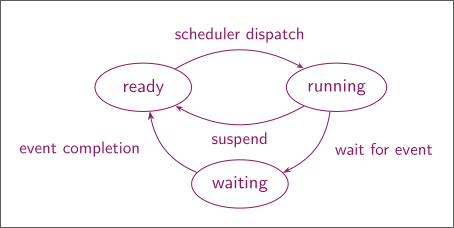
\includegraphics[scale=0.4]{2023_04_18_05_03_21.png}

\subsection{Waiting threads and Ready-Queue}
\textcolor{teal}{Waiting Threads}
\begin{itemize}
\item \textcolor{black}{Threads that are waiting are not running at all -> they are NOT waiting in a loop!}
\item \textcolor{black}{The OS instead sets the state of a thread without it doing anything}
\end{itemize} 
\textcolor{teal}{Ready Queue}
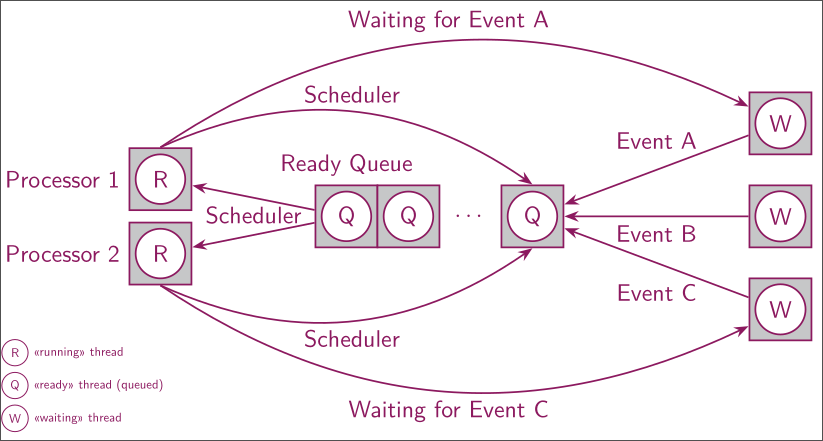
\includegraphics[scale=0.4]{2023_04_18_05_04_12.png}
\begin{itemize}
\item \textcolor{black}{All threads that are ready are in ready queue}
\item \textcolor{black}{Ready queue is not always a queue}\newline
  Scheduling might be done in a different way.
\item \textcolor{black}{new threads are usually placed in ready queue directly}\newline
  depending on the OS they might actually be placed in waiting...
\item \textcolor{black}{Threads \emph{can't directly jump into running from waiting}}
\end{itemize} 

\subsubsection{Powerdown-Mode}
\begin{itemize}
\item \textcolor{black}{Should no thread be ready to run, then the OS will put the core into standby}
\item \textcolor{black}{The sleeping core will then be awoken by the OS on interrupt and continues operation}
\item \textcolor{black}{Busy-wait, aka waiting in a loop hinders standby! This is why we should not do it!}
\end{itemize} 

\subsubsection{Types of Threads}
\begin{itemize}
\item \textcolor{purple}{I/O-heavy thread}\newline
  communicates often with I/O devices and doesn't compute much -> IO bound
\item \textcolor{purple}{processor-heavy}\newline
  doesn't communicate much with IO and computes pretty much exclusively
\item \textcolor{black}{While the difference might be vague, good systems make a difference for these to optimize performance}
\end{itemize} 

\subsection{Types of Concurrency}
\begin{itemize}
\item \textcolor{purple}{Cooperative}\newline
  Each thread decides itself when it leaves the core -> stops running
\item \textcolor{purple}{Preemptive}\newline
  The Scheduler decides when the thread will be removed from the core
\end{itemize} 

\subsubsection{Preemptive Multithreading}
\textcolor{teal}{The current thread runs until:}
\begin{itemize}
\item \textcolor{black}{waits for IO operations}
\item \textcolor{black}{waits for a resource or another thread}
\item \textcolor{black}{system timer interrupt occurs}
\item \textcolor{black}{leaves core on its own}
\item another thread with higher priority by scheduler gets into ready state
\item a new thread with higher priority by scheduler gets created
\end{itemize} 

\subsection{Parallel, "quai"parallel and Concurrent Execution}
\begin{itemize}
\item \textcolor{purple}{parallel}\newline
  all threads run parallel in realtime -> n threads require n cores
\item \textcolor{purple}{"quasi"parallel}\newline
  N threads are running on less than n cores -> this means threads will have to be scheduled\newline
  you only think they are runnin in parallel, they are actually not
\item \textcolor{red}{Concurrent} This is an overall term that can refer to either of the above!
\end{itemize} 

\subsection{Bursts}
\begin{itemize}
\item \textcolor{purple}{Core-burst}\newline
  Interval in which a thread will occupy a core fully in a parallel system
\item \textcolor{purple}{I/O Burst}\newline
  Interval in which a thread will not need the core until next event will wake the thread up again -> input event
\item \textcolor{black}{Each thread can be seen as a series of core and I/O bursts}
\end{itemize} 
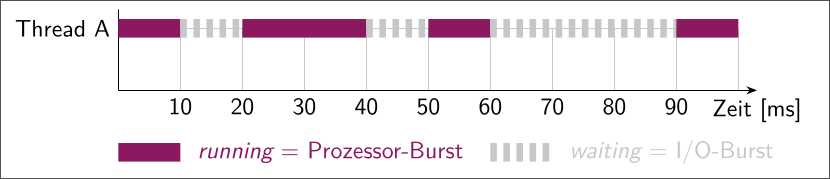
\includegraphics[scale=0.4]{2023_04_18_05_27_46.png}

\subsection{Parallel Execution as an ideal}
This means that we will never have to switch threads, this was indeed the case when there were no threads to be had.\newline
Aka inteli5 with 4 cores and that's it. This however means that there will always be wasted potential as some cores will be 100\% occupied with crap.\newline
The best case would be that we can have 500 real cores but this is unrealistic.\newline
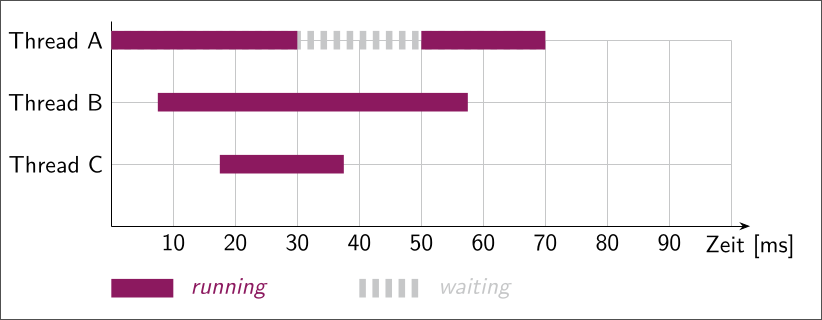
\includegraphics[scale=0.4]{2023_04_18_05_30_44.png}

\subsection{Requirements for Scheduler}
\textcolor{teal}{Note that the requirements for embedded systems and consumer devices are very different.\newline
In embedded systems you might not want a scheduler, as you know which processes will be running on there, on consumer devices you NEED scheduling as ANY process can be run on there.}\newline
Requirements from a users perspective:
\begin{itemize}
\item \textcolor{purple}{Waiting Time}\newline
  time spent by a thread in ready queue
\item \textcolor{purple}{Response Time}\newline
  time spent until response is ready after request
\item \textcolor{purple}{Turnaround Time}\newline
  time spent from start to end of a thread
\end{itemize} 
Requirements from a system perspective:
\begin{itemize}
\item \textcolor{purple}{Throughput}\newline
  Amount of threads that can be run per interval
\item \textcolor{purple}{Processor Utilization}\newline
  Core usage percentage
\end{itemize} 

\subsubsection{Conflict of interest}
The response and turnaround time will be increased by scheduling at all, but not scheduling will decrease throughput and core usage.\newline
E.g. In order to gain concurrency, you need to sacrificy some responsiveness -> last thread might need to be removed before new thread can work.\newline
Depending on the OS, or the setting of it, one or the other can be prioritized.

\subsubsection{First Come First Serve(FCFS) Scheduling}
\textcolor{teal}{This is a non-preemptive scheduling policy that does not care about thread priority or thread-task-size (how long will the task take?)}\newline
This means that this scheduling strategy will likely leave you with shitty performance.\newline
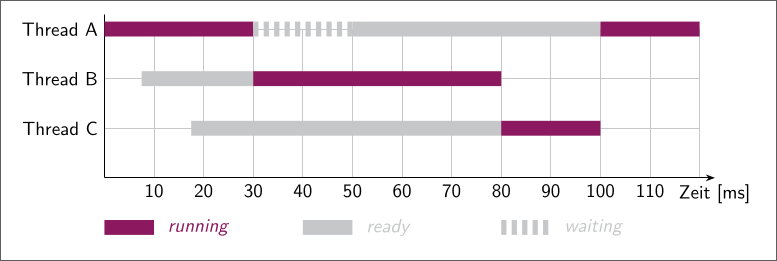
\includegraphics[scale=0.4]{2023_04_18_05_42_31.png}

\subsubsection{Shortest Job First(SJF) Scheduling Strategy}
\begin{itemize}
\item \textcolor{black}{Chooses smallest task thread first}
\item \textcolor{black}{If task size is ambiguous(more than one thread with smallest size) chooses via FCFS}
\item \textcolor{black}{Can be used cooperatively or preemptively}
\item \textcolor{purple}{The shortest thread blocks other threads minimally}
\end{itemize} 
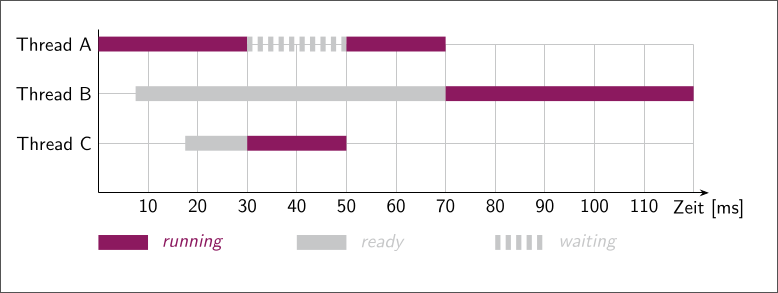
\includegraphics[scale=0.4]{2023_04_18_05_56_35.png}\newline
\textcolor{teal}{The problem with this is knowing the processor-burst -> task time\newline
There is no real way of knowing it and can therefore only be guesses.}

\subsubsection{Round-Robin Scheduling}
\begin{itemize}
\item \textcolor{purple}{Scheduler defines time slice of 10 to 100ms}
\item \textcolor{purple}{The default is FCFS, but a thread will only run as long as max time se by scheduler}
\item \textcolor{purple}{time slice size will affect performance heavily}
\end{itemize} 
30ms time slice\newline
\includegraphics[scale=0.4]{2023_04_18_05_58_23.png}\newline
10ms time slice\newline
\includegraphics[scale=0.4]{2023_04_18_06_01_05.png}

\subsubsection{Priority-Basd Scheduling}
\begin{itemize}
\item \textcolor{purple}{Each thread will receive a priority}
\item \textcolor{purple}{Threads with higher priority will be chosen over others}
\item \textcolor{purple}{Same priority will be deal with via FCFS}
\item \textcolor{purple}{SJF is a special case of this scheduling -> shorter task == higher prio}
\item \textcolor{purple}{Priorities range based on OS -> 0 to 7 or 0 to 4096 (nice level)}
\item \textcolor{red}{not to mistake with nice! -> Linux nice is per \emph{PROCESS}: -20 highest prio, 0 default, +19 lowest}
\item \textcolor{purple}{On some OS 0 is the highest priority}
\end{itemize} 

\subsubsection{Starvation}
This can happen with some scheduling systems like priority based scheduling.
Threads with lower priorities might not be able to run at all due to higher priority threads.
\textcolor{teal}{This can be improved with \emph{aging}, aka making sure threads at least get some sort of time no matter the prio.}

\subsubsection{Multi-Level Scheduling}
The OS might specify different levels for scheduling like layers: background/foreground.\newline
This means that there will be a mix of scheduling policies based on the layer the process is in, or on the priority the process is in.\newline
This helps make sure that each part of the system gets a proper amount of time to run.\newline
Queues can also be split -> high prio queue, low prio queue etc.

\subsubsection{Multi-Level Scheduling with Feedback}
\begin{itemize}
\item \textcolor{black}{Per priority one queue}
\item \textcolor{black}{Threads of higher priority queues will be preferred}
\item \textcolor{black}{exhausts a thread its time slice, then it will be placed in a lower priority -> priority - 1 }
\item \textcolor{black}{Time slices increase in lower priorities}
\item \textcolor{teal}{The effect: threads with lower bursts -> task lengths are preferred}
\end{itemize} 

\section{Scheduling in POSIX}
\subsection{Nice Value}
\begin{itemize}
\item \textcolor{purple}{Each process has a nice value}
\item \textcolor{purple}{Value ranges from -20 to +19}
\item \textcolor{purple}{Lower values == higher priority}
\item \textcolor{purple}{Default value is 0}
\item \textcolor{purple}{Only root can go below 0 with processes by default}
\end{itemize} 
\subsubsection{Nice Utility}
On Linux there is the "nice" tool that prints the current nice level or sets a new nice level:\newline
nice -n -10 command-to-run -> sets the priority 10 lower and runs command\newline
nice -> prints the nice level of process

\subsubsection{Nice function}
\begin{lstlisting}
int nice(int i)
\end{lstlisting}
\begin{itemize}
\item \textcolor{black}{adds i to the nice value of the process}
\item \textcolor{black}{returns the new nice value or -1 on error (check below....)}
\end{itemize} 
\textcolor{red}{The -1 can be an error or a nice value! Here the code to show how to get the difference:}
\begin{lstlisting}
errno = 0;
if (nice(i) == -1 && errno != 0) {
// Error
}
else {
// -1 is nice value
}
\end{lstlisting}

\subsubsection{Get Priority}
\begin{lstlisting}
int getpriority(int wich, id_t who)
int setpriority(int wich, id_t who, int prio)
\end{lstlisting}
\begin{itemize}
  \item can change priority of processes, groups or users
\item \textcolor{black}{which: PRIO\_PROCESS, PRIO\_PGRP, PRIO\_USER}
\item \textcolor{black}{who: ID of process, group, or user}
\item \textcolor{black}{getpriority() returns the nice value of the process}
\item \textcolor{black}{setpriority() sets the value of nice of the process}\newline
  returns 0 on sucess, -1 on error
\end{itemize} 

\subsection{Setting Priority of Threads}
\begin{lstlisting}
int pthread_getschedparam (pthread_t thread, int * policy,
struct sched_param * param);

int pthread_setschedparam (pthread_t thread, int policy,
const struct sched_param * param);

int pthread_attr_getschedparam (const pthread_attr_t * attr,
struct sched_param * param);

int pthread_attr_setschedparam (pthread_attr_t * attr,
const struct sched_param * param);

// note the sched_param is a struct that is not really defined
// the only thing the posix standard says is that is needs a sched_priority field.

//example usage
pthread_attr_t a;
pthread_attr_init (&a);

struct sched_param p;
pthread_attr_getschedparam (&a, &p);

// here we set the new priority of the schedule priority
// set p.sched_priority

pthread_attr_setschedparam (&a, &p);

pthread_create (&id, &a, thread_function, argument);
pthread_attr_destroy (&attributes);
\end{lstlisting}

\section{Mutexes and Semaphores}
\subsection{Producer and Consumer Problem}
This is a simple implementation to the consumr and producer problem.
\begin{lstlisting}
#define BUFFER_SIZE 16
struct item { ... };
struct item buffer [BUFFER_SIZE];

int writer = 0;
int reader = 0;

// producer thread
while (1) {
  produce_item (&buffer[writer], ...);
  int next_w = (writer + 1) % BUFFER_SIZE;
  // wait if reader is still reading next index
  while (next_w == reader) {}
  writer = next_w;
}

// consumer thread
while (1) {
  // wait if writer is writing to next index
  while (reader == writer) {}
  consume (&buffer[reader]);
  reader = (reader + 1) % BUFFER_SIZE;
}
\end{lstlisting}
Problems with this: 
\begin{itemize}
\item \textcolor{black}{Blocking wait: CPU is still used while in while loop -> useless}
\item \textcolor{black}{Does not work is multiple producers/consumers are here -> write/reader index is not atomic!}
\item \textcolor{black}{Count of elements available is unknown}
\end{itemize} 
\textcolor{teal}{If we now want to check for the amount of elements, then we can't do this immediately with --counter or ++counter\newline
this instruction is not atomic!}

\subsubsection{Non-Atomic instructions}
\begin{lstlisting}
// an instruction like
--counter;

// will turn into this assembly code
// mov rax, [counter]
// inc rax
// mov [counter], rax
\end{lstlisting}
\textcolor{purple}{After any of these assembly instructions, the CPU can be interrupted to swap to another thread etc.\newline
This means that the instruction in C is not done, leading to a potential data race!}\newline
\includegraphics[scale=0.4]{2023_04_25_05_20_56.png}\newline
This is a typical update lost problem, overwrite of an update.

\subsubsection{Critical Section}
This refers to the code segment that causes the issues -> here it is the counter increment and decrement, as well as any other non-atomic instruction.

\subsection{Synchronization}
\begin{itemize}
\item \textcolor{purple}{Mutual Exclusion:} \newline
  during a critical section, one wants other threads to not interfere with this thread -> only one thread accesses this segment
\item \textcolor{purple}{Progress:} If another thread wants to enter a critial section that is already being used, then there must be a decision on which thread enters the section next(in finite time!)
\item \textcolor{purple}{finite wait:} There must be a number N that defines how many times a thread can be overtaken, before getting a guarantee to enter the critical section
\end{itemize} 

\subsection{Atomic Instructions}
An atomic instruction is an instruction that will be done with 1 processor cycle -> can therefore not be interrupted.\newline
\begin{lstlisting}
mov [2000], rax ; atomic, naturally aligned, no shifting necessary
; in other words, this address can be divided by 8 
mov [2009], rax ; not atomic -> 2 writes necessary as not divideable by 8
; the reason: processors can write one entire byte.
; here it would write to 2009, 2010, 2011, 2012, 2013, 2014, 2015, 2016
; this means it has to write parts of 2 addresses!! 2016 is a new byte
; 2008-2015 byte 1, 2016-2023 byte 2
\end{lstlisting}
\begin{itemize}
  \item \textcolor{purple}{Modern CPUs give no guarantee that \emph{ANY} instruction definitely is atomic}
\item \textcolor{purple}{Modern CPUs will reshuffle instructions as it pleases -> this is no problem for singular threads, but can fuckup multithreaded programs}
\item \textcolor{purple}{In other words, multithreading is only possible with cooperation with hardware manufacturers}
\end{itemize} 

\subsubsection{Naive Solution: Disable interrupts}
\begin{itemize}
\item \textcolor{black}{during critical section no context switching is allowed}
\item \textcolor{black}{Ok with a single core? But not with multi core -> not thread safe}
\item \textcolor{black}{Dangerous: What happens when this thread breaks? Aka infinite loop? Or some other error? The thread can't be killed!!!}
\end{itemize} 

\subsubsection{Usage of Special Instructions}
\begin{itemize}
\item \textcolor{black}{Hardware guarantee that these instructions can't be done at the same time(even with multicore/multiCPU systems)}
\item \textcolor{black}{Locks can be done based on this system}
\item \textcolor{black}{Functions: Test-And-Set / Compare-And-Swap}
\item \textcolor{red}{In other words, YOU CANT IMPLEMENT IT IN SOFTWARE, YOU MUST USE THESE HARDWARE FUNCTIONS}
\end{itemize} 
Test-And-Set:\newline
This reads the value of from an address and sets the value to 1
\begin{lstlisting}
// NOT REAL CODE
// only example of how it works
int test_and_set (int *target) {
  int value = *target;
  *target = 1;
  return value;
}

// could then be used like this:
while (tas (&lock) == 1) {}
// do something
lock = 0;
\end{lstlisting}
Compare-And-Swap:\newline
Reads the value of the address, checks if the value is according to the expected value, and overwrite the value if it did.
\begin{lstlisting}
// NOT REAL CODE
// only example of how it works
int compare_and_swap (int *a, int expected, int new_a) {
  int value = *a;
  if (value == expected) {
    *a = new_a;
  }
  return value;
}

// usage
while (cas (&lock, 0, 1) == 1) {}
// do something
lock = 0;
\end{lstlisting}

\subsection{Semaphore}
\textcolor{purple}{The semaphore is the actual implementation of this lock!\newline
  A semaphore has a counter with a number that is \emph{always positive!}\newline
You can interact with them via special functions.}\newline
Special Functions:
\begin{itemize}
\item \textcolor{black}{Post: increments the value of the sempahore by 1}
\item \textcolor{black}{Wait: if counter is 0, thread will go to waiting until another thread increments the counter again\newline
  if counter is higher than 0, decrement and continue execution}
\item \textcolor{black}{These functions are \emph{atomic!}]}
\end{itemize} 

\subsubsection{Producer and Consumer with Semaphores}
\begin{lstlisting}
// producer
while (1) {
  // wait if consumer is in next index
  wait (free);
  produce_item (&buffer[w], ...);
  post (used);
  writer = (writer + 1) % BUFFER_SIZE;
}

// consumer
while (1) {
  // wait if writer is in current reader index
  wait (used);
  consume (&buffer[r]);
  post (free);
  reader = (reader + 1) % BUFFER_SIZE;
}
\end{lstlisting}

\subsection{Usage of Sempahores: sem\_init}
\begin{lstlisting}
// definition
int sem_init (sem_t *sem,
              int pshared,
              unsigned int value);
\end{lstlisting}
Initializes a sempahore. \newline
pshared == 0 > semaphore can only be used in this thread\newline
pshared == 1 > semaphore can be used in other threads
\, \newline
Usage:
\begin{lstlisting}
// note tis is typically a global variable!!
sem_t sem;
int main (int argc, char **argv) {
  sem_init (&sem, 0, 4);
  return 0;
}
\end{lstlisting}
Altnernative use: 
\begin{lstlisting}
// here  we create a struct that will be passed to the thread as parameter
struct T { sem_t *sem; ... };
int main (int argc, char **argv) {
  // instead of global variable, we now have a parameter
  sem_t sem;
  sem_init (&sem, 0, 4);
  // struct to pass to thread
  struct T t = { &sem , ... };
  return 0;
}
\end{lstlisting}

\subsubsection{sem\_wait and sem\_post}
\begin{lstlisting}
int sem_wait (sem_t *sem);
int sem_post (sem_t *sem);
\end{lstlisting}
\begin{itemize}
\item \textcolor{black}{Implement post and wait}
\item \textcolor{black}{return 0 on success, else -1 and error code in errno}
\item \textcolor{black}{in case of error, the semaphore will not be changed/mutated}
\end{itemize} 

\subsubsection{sem\_trywait and sem\_timedwait}
\begin{lstlisting}
int sem_trywait (sem_t *sem);
int sem_timedwait (sem_t *sem,
                   const struct timespec *abs_timeout);
\end{lstlisting}
\begin{itemize}
\item \textcolor{black}{sem\_trywait: same as sem\_wait but cancels instead of blocking if decrement not possible -> value of semaphore == 0}
\item \textcolor{black}{sem\_timedwait:} waits until either timeout reached, or wait successful
\end{itemize} 

\subsubsection{sem\_destroy}
\begin{lstlisting}
int sem_destroy(sem_t *sem);
\end{lstlisting}
Removes all memory that has been allocated for the semaphore.

\subsection{Mutexes}
A mutex has 2 states: acquired and released:
\begin{itemize}
\item \textcolor{black}{Acquire:} \newline
  if count == 0, set count to 1 and continue\newline
  if count == 1, block thread until count == 0
\item \textcolor{black}{set count to 0}
\item These are just locks
\end{itemize} 

\subsubsection{Usage}
Very easy to use:
\begin{lstlisting}
acquire (mutex);
++counter;
release (mutex);
\end{lstlisting}
\textcolor{red}{Note, mutexes are also fences, this means that noone, neither the CPU or the OS may shuffle the instruction order in a mutex.}

\subsubsection{Mutexes in POSIX}
\begin{lstlisting}
int pthread_mutex_init(pthread_mutex_t *mutex,
                       const pthread_mutexattr_t *attr);
\end{lstlisting}
attributes are optional
  \begin{itemize}
    \item \textcolor{black}{protocol: for example PTHREAD\_PRIO\_INHERIT: Mutex uses priority inheritance}
  \item \textcolor{black}{pshared: mutex can be used in other threads if set to anything other than 0}
  \item \textcolor{black}{type: Allows recursive usage or not -> with error code or without}
  \item \textcolor{black}{prioceiling: Returns minimum priority for threads that can stop the mutex}
  \end{itemize} 
Usage:
\begin{lstlisting}
// acquire (blocking)
int pthread_mutex_lock (pthread_mutex_t *mutex);

// attempt to acquire (non-blocking)
int pthread_mutex_trylock (pthread_mutex_t *mutex);

// release
int pthread_mutex_unlock (pthread_mutex_t *mutex);

// clean up
int pthread_mutex_destroy (pthread_mutex_t *mutex);

// usage in main
pthread_mutex_t mutex; // globale Variable
int main () {
  pthread_mutex_init (&mutex, 0);
  // run threads and wait for them to finish
  pthread_mutex_destroy (&mutex);
}

// usage in thread
void * thread_function (void * args) {
  while (running) {
    // Enter critical section
    pthread_mutex_lock (&mutex);
    // Perform crit. section, e.g. ++counter
    // Leave critical section
    pthread_mutex_unlock (&mutex);
  }
}
\end{lstlisting}

\subsubsection{Priority Inversion}
Problem: A thread with high priority needs a resource within a mutex, the current holder of said mutex is a thread of low priority.\newline
There is also a medium priority thread that is waiting to be scheduled.\newline
High prio thread now needs to give up it's place in order to wait for resource, but instead of getting the resource from A, B is run instead since it has higher prio than A.\newline
\includegraphics[scale=0.4]{2023_04_25_06_17_08.png}\newline
\textcolor{purple}{Solution: Priority Inheritance}\newline
This means that should thread C have to wait for a resource, then the thread holding this mutex will run with the same priority as the thread asking for the resource. \newline
In this case A would run in high prio, meaning that B will not be run:\newline
\includegraphics[scale=0.4]{2023_04_25_06_18_20.png}\newline
Legend:
\begin{itemize}
\item \textcolor{black}{purple: running}
\item \textcolor{black}{gray-dashed: waiting for resource}
\item \textcolor{black}{gray: regular waiting}
\end{itemize} 

\section{Communication and Synchronization}

\section{Programs and libraries}

\section{Graphical Overlays}

\includepdf[pages=-,scale=1]{../besys2/bsys2-typst.pdf}

\end{document}
